\documentclass[acmtog, review, anonymous]{acmart}

\usepackage{booktabs} % For formal tables
\usepackage{multirow}

% TOG prefers author-name bib system with square brackets
\citestyle{acmauthoryear}
\setcitestyle{square}


\usepackage[ruled]{algorithm2e} % For algorithms
\renewcommand{\algorithmcfname}{ALGORITHM}
\SetAlFnt{\small}
\SetAlCapFnt{\small}
\SetAlCapNameFnt{\small}
\SetAlCapHSkip{0pt}
\IncMargin{-\parindent}
\SetKwRepeat{Do}{do}{while}

\usepackage{amsmath}
\DeclareMathOperator*{\argmax}{arg\,max}
\DeclareMathOperator*{\argmin}{arg\,min}
 
% Metadata Information
\acmJournal{TOG}
% \acmVolume{9}
% \acmNumber{4}
% \acmArticle{39}
% \acmYear{2010}
% \acmMonth{3}

% Copyright
%\setcopyright{acmcopyright}
%\setcopyright{acmlicensed}
%\setcopyright{rightsretained}
%\setcopyright{usgov}
% \setcopyright{usgovmixed}
%\setcopyright{cagov}
%\setcopyright{cagovmixed}

% DOI
% \acmDOI{0000001.0000001_2}

% Paper history
% \received{February 2007}
% \received{March 2009}
% \received[final version]{June 2009}
% \received[accepted]{July 2009}

% Document starts
\begin{document}
% Title portion
%\title{OptCuts: Joint Cutting and Parameterization of 3D Surfaces} 
\title{OptCuts: Joint Optimization of Surface Cuts and Parameterization.} 

\author{Minchen Li}
% \orcid{1234-5678-9012-3456}
% \affiliation{%
%   \institution{College of William and Mary}
%   \streetaddress{104 Jamestown Rd}
%   \city{Williamsburg}
%   \state{VA}
%   \postcode{23185}
%   \country{USA}}
\email{minchernl@gmail.com}
% \author{Valerie B\'eranger}
% \affiliation{%
%   \institution{Inria Paris-Rocquencourt}
%   \city{Rocquencourt}
%   \country{France}
% }
% \email{beranger@inria.fr}
% \author{Aparna Patel} 
% \affiliation{%
%  \institution{Rajiv Gandhi University}
%  \streetaddress{Rono-Hills}
%  \city{Doimukh} 
%  \state{Arunachal Pradesh}
%  \country{India}}
% \email{aprna_patel@rguhs.ac.in}
% \author{Huifen Chan}
% \affiliation{%
%   \institution{Tsinghua University}
%   \streetaddress{30 Shuangqing Rd}
%   \city{Haidian Qu} 
%   \state{Beijing Shi}
%   \country{China}
% }
% \email{chan0345@tsinghua.edu.cn}
% \author{Ting Yan}
% \affiliation{%
%   \institution{Eaton Innovation Center}
%   \city{Prague}
%   \country{Czech Republic}}
% \email{yanting02@gmail.com}
% \author{Tian He}
% \affiliation{%
%   \institution{University of Virginia}
%   \department{School of Engineering}
%   \city{Charlottesville}
%   \state{VA}
%   \postcode{22903}
%   \country{USA}
% }
% \affiliation{%
%   \institution{University of Minnesota}
%   \country{USA}}
% \email{tinghe@uva.edu}
% \author{Chengdu Huang}
% \author{John A. Stankovic}
% \author{Tarek F. Abdelzaher}
% \affiliation{%
%   \institution{University of Virginia}
%   \department{School of Engineering}
%   \city{Charlottesville}
%   \state{VA}
%   \postcode{22903}
%   \country{USA}
% }

\renewcommand\shortauthors{Li, M. et al}

\definecolor{gray}{rgb}{0.5,0.5,0.5}
\definecolor{green}{rgb}{0, 0.6, 0}
\definecolor{orange}{rgb}{1, 0.5, 0}
\definecolor{mahogany}{rgb}{0.75, 0.25, 0.0}
\definecolor{purple}{rgb}{0.6, 0.1, 0.6}
\definecolor{darkgreen}{rgb}{0, 0.3, 0}
\definecolor{orange}{rgb}{1, 0.5, 0.}
\newcommand{\minchen}[1]{\textcolor{blue}{\textbf{Minchen: #1}}}
\newcommand{\justin}[1]{\textcolor{red}{\textbf{Justin: #1}}}
\newcommand{\alla}[1]{\textcolor{orange}{\textbf{Alla: #1}}}
\newcommand{\danny}[1]{\textcolor{purple}{\textbf{Danny: #1}}}
\newcommand{\vova}[1]{\textcolor{green}{\textbf{Vova: #1}}}

\begin{teaserfigure}
\centering
  
\includegraphics[width=\linewidth]{fig/teaser}
  \caption{Top left: three local topological operations supported in our framework; Bottom left and right: UV maps generated by AutoCuts and our method without/with bijectivity on the three man statue example visualized in 2D and on the surface.}
  \label{fig:teaser}
\end{teaserfigure}

\begin{abstract}
% context and need
Low-distortion mapping of three-dimensional surfaces to the plane is a fundamental problem in geometry processing. The intrinsic distortion introduced by such UV mappings is highly dependent on the choice of surface cuts, forming seamlines across which the mapping is not continuous.  
%Most such surfaces require cutting and distortion to produce a valid map. 
%Existing techniques largely consider seam placement and distortion minimization independently, first placing seams and then minimizing distortion; this leads to suboptimal output. Some recent attempts to address this issue ask the user to choose a potentially counterintuitive parameter weighting between seam quality and distortion and can require manual intervention to obtain a quality result. 
%\vova{Above does not encapsulate geometry images and olga's greedy seaming approach. At the same time I don't want to over-crowd abstract with these details. 
%Maybe we skip the discussion of previous work here simply motivate our approach? ``A 3D artist typically aims at a UV map that does not exceed certain distortion level (which might lead to stretching artifacts), while minimizing the seam length (which lead to discontinuities). Motivated by this observation, we propose a novel problem formulation and a joint discrete continuous optimization method...''} As an alternative, 
Parameterization applications typically require UV maps with an application-specific upper bound on distortion to avoid mapping artifacts; at the same time they seek to reduce cut lengths to minimize discontinuity artifacts. 
%Motivated by these observations,
%
We propose {\em OptCuts}, an algorithm for jointly optimizing the parameterization and cutting of a three-dimensional mesh. OPtCuts automatically minimizes seam length subject to satisfying a user-provided bound on the distortion of the mapping computed using these seams. 
%\alla{what does topology or geometry descent mean?}
%Starting with an arbitrary initial embedding, OptCuts alternates between discrete topology descent and smooth geometry descent to search for an optimal UV map strictly satisfying a specified distortion bound. 
Starting with an arbitrary initial embedding, OptCuts alternates between topology and geometry update steps that consistently decrease distortion and seam length, producing a UV map with compact boundaries that strictly satisfies a specified distortion bound. 
Aside from this user-desired bound, OptCuts requires no further parameter setting. As our examples demonstrate OptCuts automatically produces high-quality, globally bijective UV maps without any additional user intervention. We demonstrate the scalable performance of OptCuts on a wide range of challenging benchmark parameterization examples and shows that when semantic or other priors on seam placement are desired these user preferences can be directly added into the OptCuts framework.  
%
%and can generate seams whose structure is informed by a range of standard distortion measures as well as user preferences on regional seam placement.
%We also demonstrate extensions in our optimization framework enabling global bijectivity and incorporating user guidance. 
%
%\vova{Removed: ``seamlessness, and other discrete-continuous geometry processing problems''. AFAIK we are not planning to show it, correct?}
\end{abstract}


%
% The code below should be generated by the tool at
% http://dl.acm.org/ccs.cfm
% Please copy and paste the code instead of the example below. 
%
\begin{CCSXML}
<ccs2012>
	<concept>
		<concept_id>10010147.10010371.10010396.10010398</concept_id>
		<concept_desc>Computing methodologies~Mesh geometry models</concept_desc>
		<concept_significance>500</concept_significance>
	</concept>
</ccs2012>
\end{CCSXML}

\ccsdesc[500]{Computing methodologies~Mesh geometry models}

%
% End generated code
%


\keywords{geometry processing, mesh parameterization, seam placement, numerical optimization}



\maketitle

% !TeX root = OptCuts.tex

\section{Introduction}
% context
Mapping three-dimensional meshes to the plane is a fundamental task in computer graphics.  Planar images are commonly used to store reflectance functions, normals, and displacements
for the mesh, providing a domain for painting, synthesizing, and manipulating texture and geometric details. 
%Mesh parameterization is a critical task in computer graphics, with applications including texture mapping, remeshing, and detail transfer.  
%\vova{I removed non-texture apps for now, because I'm not sure if our formulation is as easy to motivate for remeshing and detail transfer.}
At its core, parameterization seeks to find a mapping from a surface---typically represented as a triangle mesh---into the plane.  To do so, parameterization tools must cope with intertwined challenges in topology and geometry:  a high-quality parameterization must cut a surface into simple %disk-shape 
patches so that each can be mapped to the plane with a reasonably small level of distortion.

Given its broad applicability, it comes as no surprise that parameterization has long been a focus of research in geometry processing.  Algorithms in this domain focus on two key aspects of the problem.  Particularly well-studied are \emph{geometric} techniques that assume a surface has already been cut into disk-topology pieces that each need to be mapped into the plane while maintaining fixed connectivity; at this point, parameterization becomes a real-valued optimization problem that seeks to minimize changes in angles and areas while maintaining local or global injectivity. Complementing these techniques, \emph{topological} algorithms find reasonable seams partitioning a surface into individual pieces that can be parameterized.  

With a few notable exceptions, previous works treat seam placement and fixed-topology mapping as separate steps in the parameterization pipeline.  This is a key drawback, as seam placement and complexity have strong bearing on the best \emph{possible} geometric parameterization of each patch.  Coupling geometry and topology, however, requires navigating between two extremes: a zero-distortion but topologically complex parameterization maps every triangle into the plane independently, while a high-distortion but topologically simple mapping might only require puncturing a few points in the input surface.
%
%\vova{not sure if we need to discuss the two extremes. I also moved some prior work discussion here.} % justin kind of likes this sentence so he decided to comment out Vova's comment :-)
%
Most previous techniques rely on heuristics for seam placement, such as computing minimal spanning tree that traverses all points with high curvature~\cite{Sheffer2002Seamster}, cutting between points of maximal distortion~\cite{Gu2002Geometry}, or greedily introducing seams during iterative flattening~\cite{BoundedDistortParam:2002}. In contrast to these methods, we propose a joint optimization framework, where discrete and continuous steps minimize the same global objective. 

% task and object    
Our parameterization algorithm, {\em OptCuts}, %couples topology and geometry. OptCuts %<--- already said this
is a jointly discrete-continuous optimization that progressively updates seam placements in between distortion minimizations to search for a locally optimal UV map satisfying an arbitrary, user-provided, distortion bound. 
%
We measure the trade-off between topology and geometry by balancing a distortion measure of choice, e.g.\ the symmetric Dirichlet energy~\cite{Smith2015Bijective}, with normalized seam length, reaching a parameterization that is near-stationary with respect to both seam placement and coordinate positions. % within a bounded number of iterations. % Justin removed --- I'm not sure this is a feature worth selling unless the bound is favorable
%\minchen{[NOTE] (Here stationary w.r.t. UV topology is only in the approximation sense, because there might still be basic topological operations that could decrease the objective but end up not chosen because it is filtered out or its locally evaluated energy decrease is not the largest one.)}

% self-weighting
%Although we acquire adaptivity to various inputs by normalizing the energy, %<-- not sure what this means
Measuring a balance between distortion and seam length has previously required a choice of a relative scaling factor between these two objectives.  From a practical perspective, it is difficult for users to choose such a coefficient. %trading off between the two. 
%Likewise, i
In practice, for high-quality solutions this balancing factor must be %somehow 
manually updated---often by user intervention during the parametrization process\ \cite{Poranne2017Autocuts}. We instead construct our coupled seam and mapping optimization as a \emph{constrained} problem. We propose to find locally minimal seam lengths for any user-set distortion bound. Treating distortion bounds as a hard inequality constraint guarantees a pre-specified level of geometric quality, while simultaneously enabling the exploration of optimal seams satisfying the bound. %In turn, o %<--- not sure what ``in turn'' means in this context
In turn, as we show below our balancing scaling factor falls directly from our model problem as the \emph{Lagrange multiplier} of the distortion bound and is thus adaptively updated directly by seeking optimality during the course of minimization process.  %directly by our optimization method.
%(Section~\ref{sec:self_weighting}).

% challenge
%Another advantage of our method is that our optimization is combinatorial, 
%
%In contrast to previous work building up a parameterization from disconnected triangle soup~\cite{Poranne2017Autocuts},  or by cutting between points of maximal predicted distortion~\cite{Gu2002Geometry,Sheffer2002Seamster}, 
%
Instead of building up a parameterization from disconnected triangle soup~\cite{Poranne2017Autocuts}, our constrained optimization method minimizes seams combinatorially, directly extending real-valued distortion minimization to the regime where seams can be incrementally introduced by cutting and removed by merging. Distortion is typically reduced by line search in UV coordinate space; we now accompany this by introducing a secondary search procedure in ``topology space'': we alternate between reducing distortion on vertex position and introducing topology changes with respect to the first-order reduction they generate in our objective formed by the local weighted sum of distortion and seam length terms. %in each topology search iteration we first find a search direction that locally decrease the objective the most (in topology step, Section~\ref{sec:topologyStep}); and then we conduct a newly derived forward-tracking line search scheme alternated with distortion minimization iterations to decide the step-size (in smooth descent step, Section~\ref{sec:descentStep}).% too much detail for intro
%\vova{Maybe the relationship to seam placement heuristics can be discussed earlier...}


% experiments
%\justin{the same 3 cites are repeated several times in the intro, not sure if it's worth maybe reducing this a it to avoid an ``us vs them'' attitude}
% \vova{I agree, and I rephrased the sentence below}
%We demonstrate our method's capabilities by comparing to AutoCuts~\cite{Poranne2017Autocuts} as well as typical classic seam cutting methods~\cite{Gu2002Geometry,Sheffer2002Seamster}. % (Section~\ref{sec:results}). 
%Given the same initial UV map, we efficiently reach identical distortion bounds with shorter seam lengths. 
We evaluate our method on a large benchmark of 3D models, demonstrating that across mesh scales and problem difficulties it successfully satisfies user-specified distortion bounds while efficiently minimizing seam length. We demonstrate that our method outperforms alternative techniques and seam placement strategies, reaching comparable distortions with fewer seams. We also show that our method is robust to tessellation/topology and scales to large inputs.%, and is stable to changes in mesh structure.~\vova{what are these changes? }

% contribution
\subsection{Contributions.}

In order to efficiently and automatically optimize both mapping and seam quality 
\begin{itemize}
  \item We propose a constrained global parameterization problem formulation to enable UV maps with specified distortion bounds and locally-minimal seam length without manual intervention. Weighting terms between distortion and seam-quality are then adapted automatically, by construction, during minimization.
\item To minimize our constrained optimization problem we present a novel algorithm, \emph{OptCuts} a joint discrete-continuous optimization that couples the minimization of seam length and metric distortion for mesh parameterization. 
\end{itemize}

Key to our method are topological search strategies as well as a dual variable treatment to search for optimal cuts with bounded distortion. Our framework naturally handles global bijectivity constraints and enables the incorporation of additional user guidance.

%We present a novel algorithm that jointly optimizes seam placement/length~\danny{should choose one term here.} and metric distortion for mesh parameterization. %, \minchen{strengthen that "seam placement" refer not only to length, but also location? and distortion can be various kinds of distortion?}. 
%%justin shortened the following sentence
%%To do so, we construct a
%Our constrained formulation %that 
%enables users to optimize UV maps with specified distortion bounds and %while gaining 
%locally-minimal seam length without manual intervention.
%% (for e.g. changing scaling terms or regularizers). \justin{i don't understand the parenthetical, seems unnecessary}
%%
%Key to our method are topological search strategies as well as a dual variable treatment searching for optimal cuts with bounded distortion. Our framework naturally handles global bijectivity constraints and incorporates user guidance. 
%\vova{we will have user guidance examples, right?}
%%\justin{rephrased previous sentence to waffle on Danny's comment for now}% \danny{We should update what we want to say here about bijectivity - seems like there's a nice observation regrading how bijectivity actually makes the optimization both better and easier but we should be clear if this is the case - if so bijectivity is more than an "ad-on" and should be a first class citizen.} 

%% !TeX root = OptCuts.tex

\section{Related Work}
Surface parameterization is a fundamental geometry processing problem that has been researched extensively~\cite{Sheffer07_ParameterizationSurvey,Hormann2008}.
Much of the literature treats surface cutting and distortion-minimizing parameterization as two separate sequential tasks. 

\paragraph{Parameterization with fixed connectivity.}
A significant body of work takes 3D surfaces with fixed connectivity and disk topology and embeds them in the plane.  The main differences between these methods is in the choice of distortion metric they seek to minimize.  While multiple methods focus on minimizing angular distortion~\cite{Floater2003,Sheffer2005ABFPP,Levy2002,Aigerman2015,Sawhney:2017}, 
others seek to produce more isometric parameterizations that account for triangle stretch~\cite{Sander2001Texture,Hormann2000MIPS,Rabinovich2017,Zhu2017BCQN,Shtengel:GOvCM:2017,claici2017isometry}. While many of these methods produce parameterizations that are not necessarily globally bijective, recent methods achieve global bijectivity by starting with a bijective map and avoiding fold-overs and global overlaps during iterative optimization~\cite{Smith2015Bijective,Jiang2017Simplicial}.
Our framework treats the mapping distortion energy as a blackbox and thus can be combined with any of the formulations above to find both the mapping and the seams necessary to bring the mapping distortion below a user desired bound. As a default we use the energy formulation of Smith et al~\shortcite{Smith2015Bijective}, which allows for efficient computation of globally bijective parameterizations.  
In Section~\ref{sec:results} we show examples of using our method in conjunction with the distortion energies proposed by \alla{ADD List}.
%
\vova{we should cite more in this paragraph above (e.g., missing hughes hoppe papers} \alla{Added Sanders, ARAP would be good too}

Starting with the work of Kharevich et al.~\shortcite{Kharevich} a number of seamless or globally continuous parameterization approaches had been proposed~\cite{pgp,others}. These methods can use as a starting point either closed meshes or meshes with relatively short boundaries; they reduce distortion by using either pre-computed or algorithmically introduced cone singularities, i.e.\ discrete points on the surface where the mapping is discontinuous. While these methods have proven useful for applications such as quad meshing, the 2D embedding, or atlas, they generate tend to be less suited for signal storage. Thus most signals defined over 3D assets in digital media settings (movies, games, etc.) are typically stored as traditional atlases with discontinuous seams.  

\paragraph{Separate Cut Computation.}
Multiple frameworks exist that cut or segments meshes prior to parameterization~\cite{Sheffer2002Seamster,Julius2005D,Snyder2003Multi,Levy2002,needMore}.
Since the cutting is done before the parameterization, they rely on proxy metrics as a predictor of anticipated mapping distortion. Consequently, achieving a desired distortion bound using these tools requires trial and error, as users need to provide the right proxy parameter thresholds that result in the amount of distortion they ultimately want to achieve. By combing the two tasks we allow users to control the tradeoff between mapping distortion and seam length directly. 

\paragraph{Simultaneous Cutting and Parameterization.}
A handful of methods directly consider mapping distortion when making cutting choices. 
Sorkine et al.~\shortcite{BoundedDistortParam:2002} parameterize the surface triangle-by-triangle, introducing cuts when distortion exceeds user-prescribed bound. Due to the method's locality it tends to introduce longer than necessary seams to achieve a given bound~\cite{Hormann2008,Poranne2017Autocuts}. 
Gu et al.~\shortcite{Gu2002Geometry} use an incremental approach, where starting with a given parameterization they  repeatedly introduce cuts connecting the current boundary with distortion maxima in the current parameterization.  This approach works well in the presence of a few distortion extrema, but becomes less effective when the distortion is more evenly distributed (Figure~\ref{fig:fig:comp_GI},left). Our framework performs equally well in both scenarios.  

%\vova{do multi-chart geometry images~\cite{Snyder2003Multi} and geometry images use the same strategy? } 
% \alla{no}
%%
%These heuristics do not perform well if no such obvious points exist, e.g.\ once distortion is distributed near-evenly across many surface points. Our framework in contrast searches for minimal cut elongation or shrinking steps that reduce a joint objective, and thus we expect it to be more efficient in such settings (Figure~\ref{cases where there are not many obvious extremal points}).
%%
%One can also parameterize the surface triangle-after-triangle introducing cuts when distortion exceeds user-prescribed bound~\cite{BoundedDistortParam:2002}. 
%%
%All of these seam cutting strategies, however, follow greedy heuristics and do not provide a well-defined global objective that balances between the introduced cuts and overall distortion. 

%related methods:\\
%AutoCuts~\cite{Poranne2017Autocuts}\\
%%SeamCut~\cite{Lucquin:2017}\\ % interactive
%
%%Seams, due to its discontinuous property, is not intuitive to be considered in traditional distortion minimization frameworks.
%Due to discontinuities that occur when seams are introduced or removed, it is not intuitive to consider optimization of seam topology in the context of traditional frameworks for minimizing distortion during mesh parameterization.
%%
%\justin{couldn't follow this sentence (what does ``efficient'' or ``sparse'' mean in this context and what does it have to do with L2?):}
%Moreover, for seams to be efficient, it needs to be sparse, which is another challenge for optimizing it with L2-type distortion energies.
%\minchen{RE:Justin: what about changing the sentence to:}Distortions are usually measured with smooth L2-type energy, where at local minimum the residual distortions are distributed evenly over the trangles. This is essentially different from the behavior of seams, which is either glued together or separated. Hence, approximating seam topology using UV coordinates would require nonsmooth energy to enforce sparsity structure, which makes the problem ill-conditioned.

AutoCuts~\cite{Poranne2017Autocuts} optimizes an energy function defined as a weighted average of seam length and mapping distortion metric. The AutoCuts optimization procedure progressively builds up a parameterization starting from a triangle soup, jointly improving connectivity and distortion via homotopy optimization. \vova{need to be a bit careful about initialization, because they show two in their paper}
\alla{agree - someone needs to read carefully and update}
The method is targeted to user-assisted parameterization and provides multiple ways for users to interact with the system. Our framework is designed for settings where users want to obtain parameterizations automatically, but it still allows a few mechanisms of user control discussed in Section~\ref{sec:results}.  
The use of a formulation that weighs two quantities with very different scale in an automatic setting is challenging as users have little intuition as to which balance will achieve the parameterization they envision. Our approach of allowing users to provide a hard bound on distortion enables them to easier communicate their intent. 
%
%We observed that i
%\alla{delted all claims below unless we can demonstrate them}
%While their method is among the first to optimize parameterization topology and geometry simultaneously, 
%initially placing seams on all the edges introduces unneeded degrees of freedom and unnecessary computational expense:  Most of the triangles remain attached to their neighbors after their optimization procedure converges. Also, since their seam placement highly depends on the homotopy path, AutoCuts relies on user guidance to obtain good results, e.g.\ for parameter tuning, cut suggestion, and patch movement. 
%\danny{Here or elsewhere we should also add the observation that a full triangle soup initializer requires an awful lot of extra (and generally unnecessary) work to glue everything back together...}%\justin{how's the above?}

%Our framework is different from well-known seam cutting algorithms like Geometry Images~\cite{Gu2002Geometry} and Seamster~\cite{Sheffer2002Seamster}, in which the core idea is to locate points of maximal currently predicted distortion and to add cut paths toward them. These heuristics do not perform well if no such obvious points exist, e.g.\ once distortion is distributed near-evenly across many surface points. Our framework in contrast searches for minimal cut elongation or shrinking steps that reduce a joint objective, and thus we expect it to be more efficient in such settings (Figure~\ref{cases where there are not many obvious extremal points}).

%\vova{not sure if we need the paragraph below.}
%
%Although OptCuts does not require user assistance, it still allows users to communicate preferences on regional seam placement through edge weight painting (Figure~\ref{fig:edge_weight_painting}), which is more in-line with common practices used by UV artists.  In addition, it can work with ``bespoke'' distortion energies when necessary. For example, it creates different set of seams that benefit conformality if the objective function penalizes conformal distortion (Figure~\ref{results of our method with conformal distortion energy}).


\section{Related Works}

related methods:
AutoCuts~\cite{Poranne2017Autocuts},
Seamster~\cite{Sheffer2002Seamster},
geometry images~\cite{Gu2002Geometry},
Multi-chart geometry images~\cite{Snyder2003Multi},
D-Chart~\cite{Julius2005D}


components:
Bijective parameterization with free boundaries~\cite{Smith2015Bijective},
projected Newton~\cite{Teran2005Robust},
MIPS~\cite{Hormann2000MIPS},

% !TeX root = OptCuts.tex

\section{Problem Statement}
%\minchen{As Vova suggested, describe Self-Weighting as our main formulation before Joint Discrete-Continuous Search, so does Abstract, Introduction, and Section 4 and 5.}
% \danny{Also took a pretty heavy pass at re-organizing this section and the next.}

Given an input triangle mesh $M=(V,F)$ of a three-dimensional surface with vertices $V$, and faces $F$, we seek its UV embedding with connectivity $T^*=(V_{T^*}, F_{T^*})$ and a corresponding two-dimensional embedding of vertex coordinates, $U^* \in \mathbb{R}^{2 |V_{T^*}|}$, that locally optimizes the constrained parametrization problem
%
\begin{align}
	\min_{T,U} E_s(T) \quad s.t. \quad E_d(T,U) \leq b_d\ \ \text{and}\ \ (T, U) \in \mathcal{I}.
	\label{eq:p1}
\end{align}
%\justin{Might be worth mentioning in a sentence what your representation of $T$ is} \minchen{I haven't thought about defining $T$ explicitly. If needed, it can be a vector of boolean variables representing whether each edge on the 3D surface is a seam edge, subject to manifold mesh constraints.}
%\vova{Binary value over edges requires additional post-process to identify which of two vertices are duplicated and which triangles they should be assigned to. 
%Why not just define a new mesh $(V_T, F_T)$ and a bijective map $f_T: F \rightarrow F_T$?}\danny{My suggestion is that we stick as closely as possible to the rep used in Minchen's code - I've asked him what he uses - we can monge that into text once he replies.} \minchen{Similar to Vova said, I simply use the vertex indices of each face to represent topology as what .obj file does. Should we mention it here or in the implementation section?}
%
Here $V_{T^*}$ is a superset of $V$ with possibly duplicated vertices, and $F_{T^*}$ is the set of original faces indexed into this new set of vertices. We use $\mathcal{I}$ to define the set of \emph{either} locally injective \emph{or} globally bijective UV maps; in the following we will first initially focus on the locally injective set and then discuss the extension to globally bijective maps (Section~\ref{sec:bijectivity}). Energies $E_s$ and $E_d$ respectively measure seam quality (length) and map distortion while $b_d$ is a user-specified \emph{upper bound} on the acceptable distortion of the generated map. This optimization is always feasible as in the limit having all triangles separated would allow for zero distortion. %\danny{If we truly want to make bijectivity a first-class component of our method (I'd suggest we do then we should add the bijectivity constraint to the optimization problem statement above and also the derivation that follows - happy to do this once we decide.}

In general, distortion measures are smooth albeit \emph{nonconvex}, while seam length measures are \emph{nonsmooth} as they increase by discrete amounts when interior mesh edges are cut along or seam edges are merged. Hence, generic optimization techniques cannot be easily applied to our setting; instead we need to design a tailored optimization method that addresses both challenges.

%
% e.g. symmetric Dirichlet, MIPS, etc, to measure distortion over the mapped domain. In what follows, for simplicity we largely focus on the symmetric Dirichlet energy and defer examples with other distortion measures for our results to Section\ \ref{}.

%Given an input triangle mesh $M$ of a 3D surface with $n_p$ vertices and its initial UV map with topology $T^0$ and coordinates $U^0 \in \mathbb{R}^{2n_p}$, we automatically search for
%\[ \argmin_{T,U} L(T,U) \]
%where $L(T,U) = E_s(T) + \lambda E_d(T,U)$ is the total energy combining both seam energy $E_s$ and distortion energy $E_d$ with a balancing factor $\lambda \in \mathbb{R^+}$. Notice that usually $E_d$ is smooth, while $E_s$ is defined to be non-differentiable, which gives us a discrete-continuous problem.

\subsection{Dual Objective}
As a first step toward solving the problem at hand, we construct the Lagrangian for (\ref{eq:p1})  % no need to cite the definition of a Lagrangian
\begin{align}
	L(T,U,\lambda) = E_s(T) + \lambda(E_d(T,U) - b_d),
	\label{eq:L}
\end{align}
%
to form the equivalent saddle-point problem~\cite{Bertsekas:2016:NOP} defined over primal variables $T,U$ and dual variable $\lambda$:
%
\begin{align}
	\min_{T,U} \max_{\lambda\geq0} L(T,U,\lambda).
	\label{eq:p2}
\end{align}
%
Here $\lambda \in \mathbb{R_+}$ is the Lagrange multiplier for our distortion bound. On examination the Lagrangian $L$ can be seen as a multi-objective balancing between distortion and seam quality as dictated by $\lambda$. Here, however, $\lambda$ effectively applies a local scaling between the seam and distortion terms that is implied %directly and automatically given 
by the user-specified distortion bound. As we iterate to solve  \eqref{eq:p1}, $\lambda$ will grow when we threaten to violate our distortion bound  prioritizing distortion minimization; similarly, $\lambda$ will decrease toward $0$ when our bound is strictly satisfied to prioritize seam quality.


\subsection{Embedding Energy}
Concretely we formulate our seam-quality energy as the normalized total seam length
\begin{align}
E_s 
%= E_{SL} 
= \frac{1}{\sqrt{(\sum_{t\in\mathcal{F}} |A_t|)/\pi}} \sum_{i \in \mathcal{S}} |e_i|
\end{align}
where $\mathcal{S}$ is the set of all seam edges on the input surface and $|e_i|$ is the length of edge $i$ in the input mesh.
We measure distortion over the mapped domain using the symmetric Dirichlet energy~\cite{Smith2015Bijective} normalized by surface area~\footnote{For simplicity we focus on symmetric Dirichlet here; alternate distortion energies follow similarly.}, 
\begin{align} 
E_d 
%= E_{SD} 
= \frac{1}{\sum_{t\in\mathcal{F}} |A_t|} \sum_{t\in\mathcal{F}} |A_t|(\sigma_{t,1}^2 + \sigma_{t,2}^2 + \sigma_{t,1}^{-2} + \sigma_{t,2}^{-2}),
\end{align}
where $\mathcal{F}$ is the set of all triangles, $|A_t|$ is the area of triangle $t$ on the input surface, and $\sigma_{t,i}$ is the $i$-th singular value of the deformation gradient of triangle $t$.
%We picked this distortion measure among other choices since it efficiently balances between angle and area distortion and preserves local injectivity, but our method can be used with other metrics as well.
%\vova{should we that seam penalties and distortion measure choices are analogues to AutoCuts (but our objective is defined differently?)}
%Also note that our seam penalty and distortion measures are analogous to those used in AutoCuts~\cite{Poranne2017Autocuts}, although the way we combine these terms is different.  
%
%With the energies normalized, $L$ is invariant to coordinate scale and resolution for meshes with the same shape. %\danny{removed as this claim - for mesh resolution it is not true - certainly helps for scaling though.}


\subsection{Adding Global Bijectivity}
Most applications or UV embeddings  require global bijectivity. Following the observations of Jiang et al.'s\ \shortcite{Jiang2017Simplicial} we realize this additional constraint on our mapping by first triangulating the outer, void, regions of each iteration's updated UV map and then augmenting our distortion energy $E_d$ with an additional term, \emph{not included in the distortion bound constraint}, that prevents the added void-space triangles from collapsing during each optimization iteration. For details see Section\ \ref{sec:bijectivity}. 
%As these constraints are implicitly encoded in our constraint. The additional objective terms are not added as a term to the distortion bound. Moreover, our framework stays the same when solving this extended problem.

% \danny{Moved and reorganized a good portion of what was here to the next section.}



%%%%%%%%%%%%%%%%%%%%%%%%%%%%%%%%%%%%%%%%%%%%%%

%\paragraph{Joint Discrete-Continuous Search}
%
%Instead of trying to solve an ill-conditioned real-valued optimization by approximating $T$ with $U$ \cite{Poranne2017Autocuts}, we alternatingly optimize $T$ (in topology steps) and $U$ (in descent steps), augmenting the continuous search with a discrete topology search (Section~\ref{sec:DCSearch}).
%
%Descent steps deal with the continuous search
%$\min_U E_d$
%where $T$ is fixed and Newton-type method is applied (Section~\ref{sec:descentStep}).
%Topology steps deal with the discrete search (Section~\ref{sec:topologyStep}) where a neighboring topology is searched based on the first-order reduction it would cause in $L$.
%While each descent step is one complete Newton-type iteration with back-tracking line search, we use a sequence of topology steps alternated with descent steps to perform a forward line search in topology space: a search direction is first decided and then the step size is increased to ensure sufficent energy decrease.
%
%Given a topology change, we evaluate the first-order reduction of $L$ it would cause by minimizing $E_d$ only on the local stencil of the edited seam edge and combine it with the $E_s$ change. Experiments demonstrate that this is efficient and sufficient for always editing the seams reasonably and sustainably (Section~\ref{sec:results_exp}).
%
%Since we ensure $L$ to be monotonically decreased in both the descent steps and topology steps, we can easily prove that a near-stationary point can be reached for any input within a bounded number of alternations (Section~\ref{sec:convergence}).

%\paragraph{Self-Weighted Objective}
%
%To automatically decide $\lambda$ and enable users to directly control the distortion they expect for the output UV map, we formulate a constrained optimization seeking to minimize seam energy $E_s$ subject to user-specified distortion bounds $b_d$:
%\[ \min_{T,U} E_s(T) \quad s.t. \quad E_d(T,U) - b_d \leq 0 \]
%Introducing $\lambda$ as a dual variable gives us
%\[ \min_{T,U} \max_{\lambda \in \mathbb{R^+}} E_s(T) + \lambda(E_d(T,U) - b_d) \]
%We solve it by adding a regularization term to make it smooth for $\lambda$, and alternatingly updating dual variable $\lambda$ and primal variables $T$ and $U$ (Section~\ref{sec:self_weighting}).
%
%The challenge here is that the initial embedding we start from is usually with high distortion, thus infeasible, and the quality of the output seams is highly affected by the $\lambda$ updating scheme. \minchen{[TODO] briefly describe what we do after finalized}
 
 %\danny{I haven't commented it the next paragraph but would suggest we: 1. remove this next paragraph from paper, 2. make bijection a main part of the algorithm and 3. move everything else to future work (if we don't do it) or results (if we do get to it).}\justin{cool w me} 

% \vova{
% I think the structure is a bit confusing (e.g., problem is not entirely defined in ``problem statement'', since we lack precise energy formulation, self-weighted objective talks about outer-look  (alg 1) and then about self-weighting. 
% %
% I propose the following structure: \\
% Section 3: first three paragraphs followed by ``dual objective'' (i.e., exclude "concretely we formulate ...)\\
%  - then write ``energy definition'' paragraph (from sec 5.3 and ``concretely we formulate'' paragraph) \\
 % - then write ``energy with global bijectivity'' paragraph (start ``for most texture applications one needs to ensure global bijecivity, we incorporate this into our energy following Jiang2017...'') \\
 % - [this and below is optional] then write ``optimization framework'' paragraph with Algortihm 1 and first paragraph from section 4. Here reference section 4 for dual update and section 5 for primal update. \\
 % - Note due to the last paragraph, we might change this section from ``Problem Statement'' to ``Optimization Framework''. Alternatively, we can have a separate section (between current 3 and 4, titled ``optimization framework'')\\
 % - Initialization (obtaining $T^0, U^0$ is not described anywhere. We should at least mention it in ``optimization framework'' part of the text. \\
% Section 4: rename into Dual Update \\
% Section 5: rename into Primal Update
% }

%\vova{I suggest we consistently use paragraphs or subsections across sec 3, 4, 5}

% !TeX root = OptCuts.tex

\section{Optimization Framework for OptCuts}

We solve the constrained optimization problem (\ref{eq:p1}) by recasting it as a saddle-point problem (\ref{eq:p2}). 
We start from an initial, valid UV map $(T^0, U^0)$ and set our dual variable as $\lambda^0 = 0$. OptCuts then iteratively alternates between primal solves designed to improve geometry, $(T, U)$, and dual solves updating our multiplier, $\lambda$,  encoding the new balancing term between distortion and seam quality for the next primal solve we take. See Algorithm 1.

%\begin{algorithm}[!h]
%\SetAlgoLined
%\KwData{$M$, $T^0$, $U^0$, $b_d$}
%\KwResult{$T^*$, $U^*$}
%
%$\lambda^0 \leftarrow 0$, $k \leftarrow 1$\;
%
%\Do{either primal or dual not converged}{ 
%  $\lambda^{k}$ $\leftarrow$ dualUpdate($T^{k-1}$, $U^{k-1}$, $b_d$, $\lambda^{k-1}$); // Section~\ref{sec:dualUpdate}\\
%
%  $(T^{k}, U^{k})$ $\leftarrow$ primalUpdate($M$, $T^{k-1}$, $U^{k-1}$, $\lambda^{k}$); // Section~\ref{sec:primalUpdate}\\
%
%  $k \leftarrow k + 1$\;
%} 
%$(T^*, U^*)$ $ \leftarrow$ $(T^{k-1}, U^{k-1})$\; 
%
%\caption{OptCuts}
%\label{alg:selfWeight}
%\end{algorithm}

%\danny{Suggest moving this to our implementation section 
%\subsection{Initialization}
%To obtain an initial UV map for an input surface, we map its initial seam to a circle preserving edge length and parameterize the rest of the vertices through Tutte embedding with uniform weights.
%
%We compute initial seams for different surfaces according to their topology and geometry. For disk-topology surfaces, we simply pick their longest boundary as the initial seam. For genus-0 closed surfaces, we randomly pick 2 connected edges as the initial seam. \minchen{[TODO] change to curvest one point cut or farthest point cut if they are better} For high-genus surfaces, we follow Crane et al.~\shortcite{Crane:2013:DGP} to detect homology generators and connect all of them as the initial seam \minchen{[TODO]}.
%
%We simply start by ignoring the distortion constraints with $\lambda$ set to $0$, and let our dual update to modify $\lambda$ according to the intermediate distortions.


\subsection{Primal Update}
\label{sec:primalUpdate}
Our $k$th primal update is a joint discrete-continuous search over variations in geometry to minimize the weighted sum of seam length and distortion energies in our Lagrangian (\ref{eq:L}). We hold the current iterate's dual variable, $\lambda^k$, fixed and initialize with the last iterate's geometry $(T^{k-1}, U^{k-1})$.

%Rather than trying to approximate $T$ with non-smooth energies of $U$ and solve a potentially ill-conditioned real-valued optimization, we alternate local optimizations over $U$ and then $T$ in each inner iteration and obtain $(T^{k+1}, U^{k+1})$ when both are converged (Algorithm~\ref{alg:DCSearch}).

We initially experimented with solving our primal problem by approximating topology change with non-smooth energies on duplicated vertices of the input mesh, in a manner similar to AutoCuts\ \cite{Poranne2017Autocuts}. Unfortunately, this quickly led to problems with strongly ill-conditioned real-valued optimization and prevented scaling to larger meshes. 

To counter these challenges we directly optimize in alternating inner steps searching over changes in topology $T$ and vertex positions $U$. These inner iterations loop until we 
%converge to a minimizer of the Lagrangian at the fixed $\lambda^k$, 
reach a stationary point, 
giving us iterate $k$'s newly updated geometry $(T^{k}, U^{k})$; see Algorithm 1.% and Section\ \ref{sec:topologySearch}. 

%\danny{Minchen: correct me if I'm wrong but I don't believe you employ an actual convergence measure - you simply wait until the $(T,U)$ remain unchnged by further iterates. Is this correct?} \minchen{Correct. We simply stop the discrete-continuous alternations when continuous search converges since it also means topology search won't go further in the current direction. For continuous search, besides gradient tolerance, I also have a relative energy decrease tolerance ($10^{-6}$). It is not because we have troubles converging to small gradient, which is actually not necessary. Setting extra tolerance on relative energy decrease is more stable than using larger gradient tolerance.}

%\begin{algorithm}[h]
%\SetAlgoLined
%\KwData{$M$, $T^{k}$, $U^{k}$, $\lambda^{k+1}$}
%\KwResult{$T^{k+1}$, $U^{k+1}$}
%$i \leftarrow 1$, $T^{k,0} \leftarrow T^{k}$, $U^{k,0} \leftarrow U^{k}$\;
%$\delta^{k,0} \leftarrow 0$\;
%\Do{either step is not converged}
%{
%	($T^{k,i}$, $U_a^{k,i-1}$) $\leftarrow$ topologyDescentStep($M$, $T^{k,i-1}$, $U^{k,i-1}$, $\delta^{k,i-1}$, $\lambda^{k+1}$); // Section~\ref{sec:topologySearch}\\
%	($U^{k,i}$, $\delta^{k,i}$) $\leftarrow$ smoothDescentStep($M$, $T^{k,i}$, $U_a^{k,i-1}$); // Section~\ref{sec:descentStep}\\
%	$i \leftarrow i+1$\;
%}
%$T^{k+1} \leftarrow T^{k,i-1}$, $U^{k+1} \leftarrow U^{k,i-1}$
%\caption{Primal Update $k+1$}
%\label{alg:DCSearch}
%\end{algorithm}

Each vertex step of the primal update performs a single iteration of Newton-type, smooth descent with line-search towards minimizing our distortion energies over vertices $U$ while holding topology, $T$, fixed. As our distortion energies, including symmetric Dirichlet, are generally nonconvex we employ the projected-Newton\ \cite{Teran2005Robust} approximation of the Hessian. This is then coupled with 
%For more details see Section \ref{sec:imp}.
search of topology changes to form a customized discrete-continuous topology search method. We defer discussion of the details of this component to Section~\ref{sec:topologySearch}.
%

%Each vertex update step performs a single iteration of Newton-type, smooth descent with line-search towards minimizing our distortion energies over vertices $U$ while holding topology, $T$, fixed. As our distortion energies, including symmetric Dirichlet, are generally nonconvex we employ the projected-Newton\ \cite{Teran2005Robust} approximation of the Hessian here. For more details see Section \ref{sec:imp}.
%%
%%The continuous search is peformed in each smooth descent step, where we conduct a complete Newton-type iteration with backtracking line search towards minimizing distortion $E_d$ over vertices $U$ while holding topology, $T$, fixed (Section~\ref{sec:descentStep}).
%%
%Our topology step requires the construction of a custom discrete topology search method. We defer discussion of the details of this component to Section~\ref{sec:topologySearch}.
%%
%The discrete topology search is performed in each topology descent step by querying a set of neighboring topologies and changing to the one with largest first-order reduction in $L$ if this reduction is prominent (Section~\ref{sec:topologySearch}). 
%

%By thresholding topology changes using the energy decrease of the last smooth descent step, we always proceed either the discrete topology search or the continuous search that decreases $L$ more.\justin{didn't follow previous sentence.}

\subsection{Dual Update}
\label{sec:self_weighting}
\label{sec:dualUpdate}

% Our overall minimization is inequality constrained with a specified upper bound $b \in \mathbb{R}_+$ on distortion. \justin{I moved a parenthetical to a Minchen comment assuming he'll write it more formally}\minchen{(L2 norm on SD  energy for now - pretty easy to modify to an extremal measure if we want later on.)}

%

%In this section we describe the update for the dual variable $\lambda^k$ given the current UV map $(T^{k-1}, U^{k-1})$.


Our Lagrangian in (\ref{eq:p2}) is nonsmooth in $\lambda$. When we exceed the distortion bound, i.e., $E_d(T,U) > b_d$, we have $\lambda = \infty$; when on boundary of the feasible set, $E_d(T,U) = b_d$, we have a finite $\lambda \in \mathbb{R_+}$; and finally, in the strict interior of the set of feasible distortions, we have $\lambda = 0$. While these conditions nicely characterize optimality, we need a way to iterate on $\lambda$ towards the solution in a smooth and robust manner irrespective of whether we are locally exploring a feasible or infeasible distortion. 

At iteration $k$ we thus smoothly approximate the multiplier's behavior by adding a simple quadratic regularizer to the Lagrangian. This keeps the updated multiplier \emph{proximal} to the previous iterate's estimate via Powell's extension\ \cite{Powell73} of the Augmented Lagrangian to the inequality constrained setting,
%\begin{align}
%	\min_{T,V} \max_{\lambda \geq 0} E_{s}(T^{k-1}) + \lambda \big( E_{d}(T^{k-1}, U^{k-1}) - b_d\big) - \frac{1}{2\kappa} (\lambda- \lambda^{k-1})^2. 
%\end{align} 
\begin{align}
\label{eq:al}
	\min_{T,V} \max_{\lambda \geq 0} E_{s}(T) + \lambda \big( E_{d}(T, U) - b_d\big) - \tfrac{1}{2} (\lambda- \lambda^{k-1})^2. 
\end{align} 
At each iteration, to find $\lambda^k$ we simply fix vertices and topology to  $(T^{k-1},U^{k-1})$. Optimality of (\ref{eq:al}) then gives us our corresponding dual update in closed form
%\begin{align}
%\lambda^{k} \leftarrow \max\big(0,\kappa \big( E_{d}(T^{k-1}, U^{k-1}) -b \big) + \lambda^{k-1}\big).	
%\end{align}
%We simply use $\kappa = 1$ for all inputs throughout our paper, since it is appropriately small that would not overly change the Lagrangian.
\begin{align}
\lambda^{k} \leftarrow \max\big(0,\big( E_{d}(T^{k-1}, U^{k-1}) -b_d \big) + \lambda^{k-1}\big).	
\end{align}






%When distortion is a since it does not take into account the fact that we might start away from feasibility and want to iteratively improve both our primal variables $(T, U)$ and our dual variable $\lambda$. To smoothly update to a current $\lambda^{k}$ in iteration $k$ from a previous estimate $\lambda^{k-1}$, we add a simple quadratic regularizer $R(\lambda,\lambda^{k-1}) = \frac{1}{2\kappa} (\lambda- \lambda^{k-1})^2$ \justin{to what?} to make sure $\lambda$ iterates behave reasonably. \justin{Right now previous sentence sounds quite heuristic; can you cite an optimization algorithm that does this?} In practice, we simply set $\kappa = 1$.
%
%For iteration $k$ this gives us 
%\[ \min_{T,V} \max_{\lambda \geq 0} E_{s}(T^{k-1}) + \lambda \big( E_{d}(T^{k-1}, U^{k-1}) - b_d\big) - \frac{1}{2\kappa} (\lambda- \lambda^{k-1})^2 \]
%which can be solved in closed form as
%\[ \lambda^{k} \leftarrow \max\big(0,\kappa \big( E_{d}(T^{k-1}, U^{k-1}) -b \big) + \lambda^{k-1}\big) \]
%
%\danny{(Notice that throughout the above we can define a progressive $\lambda$ without needing to employ subgradients to reason about nonsmoothness in our sparsity energy.)}\justin{didn't follow this, not sure it's needed}



% \vova{The section below seem to be concerned with convergence of Alg 1, which is beyond self-weighted objective, IMHO... 
% It is also confusing that there a subsection 5.7 on convergence...}
%\subsection{Convergence}
%
%Our primal update converges when the UV map reaches the local minimizer of $L$ in both continuous and discrete searches. Similar to standard continuous search, our discrete topology search also converges at a local minimum, but in topology space, where changing to all neighboring topologies can not decrease $L$. Since we ensured monotonic decrease in $L$ over both the smooth and topology descent steps, we can prove that a near-stationary point with respect to both $T$ and $U$ can be reached for any input within a bounded number of alternations given a fixed lambda (Section~\ref{sec:convergence}).
%
%Theoretically, the dual update converges in two situations: either at $\lambda^* = 0$ when the primal minimizer $(T^*, U^*)$ is inside the feasible region ($E_d(T^*, U^*) < b_d$) with no seams, or at some $\lambda^* > 0$ with $(T^*, U^*)$ on the boundary of the feasible region ($E_d(T^*, U^*) = b_d$). However, for the latter case, since there is only a finite number of configurations of $T$, the near stationary $E_d$'s may not be exactly equal to $b_d$. Instead of setting a relatively large tolerance for detecting convergence, we stop when it first tries to violate distortion bound $b_d$ from being feasible. \justin{this was kind of vague; is it in the pseudocode?}


% !TeX root = OptCuts.tex

\section{Coupled Discrete-Continuous Descent}
\label{sec:topologySearch}
To perform our primal update, we seek to minimize the Lagrangian over both continuous changes in vertex positions \emph{and} discrete changes in topology. 
%
To optimize over topology we could potentially perform exhaustive search over the graph of all possible mesh changes. This approach, however, is intractable for any practical mesh size. 
%
Instead, we devise a local search algorithm for topological updates inspired by the standard descent process of optimizing a smooth energy over vertex positions. 

%
%Instead, we begin by recalling the standard process of optimizing a smooth energy solely over vertex DoFs. In such cases, each iterate generally forms a localized approximation of the minimized energy \justin{didn't understand previous phrase} and then uses it to propose a candidate direction for decrease. Then, since finding such a direction is expensive, we search along the proposed direction to ensure a significant decrease in energy (and not increase). 
The descent standard process is to formulate a local approximation to the energy function, use it to estimate the direction for the gradient descent step, and then search along the proposed direction to find the step magnitude that ensures significant decrease in energy. 
%
We extend this process to include search over discrete variations in topology. In analogy to seeking a continuous search direction, at the start of each new primal solve we will build many localized energy approximations to search for a likely candidate mesh operation to repeatedly propagate topology change, i.e., cutting or merging, over our UV mesh. Each inner iterate of the primal solve will successively apply this operation in combination with standard smooth descent to explore discrete-continuous descent until no further progress is made.% and so a primal update is found.    %<-- doesn't seem needed

In the remainder of this section we formulate the energy model that is used to evaluate the candidate topology operations (Section ~\ref{sec:topology_energy}), 
enumerate the topology operations used in our algorithm (Section~\ref{sec:topology_ops}), explain how we find the search direction (Section~\ref{sec:descent_op}), and iteratively explore the identified direction (Section~\ref{sec:topology_search}).

\subsection{Energy Model for Topology Updates}
\label{sec:topology_energy}
We next devise an approximate energy model to efficiently estimate the effect of a potential topological change. 
To keep our notation simplified, in the following we use $i$ or $j$ to index the inner loop of the primal update and $k$ for indexing the outer loop.
At each outer iterate $k$, the optimal Lagrangian for any proposed topology $T^i$ is  
\begin{align}
\ell(T^i) = \min_{U} L(T^i, U) = E_s(T^i) + \lambda^k \min_{U} E_d(T^i, U).
\end{align}
Then, for any valid topology-changing operation, $o^{i,j}:T^i \rightarrow T^j$, the resultant change in Lagrangian is $\Delta \ell(o^{i,j}) = \ell(T^j) - \ell(T^i)$. We seek a valid operation that will produce large decrease in the Lagrangian.


Since minimizing over $U$ for every potential topology change is intractable for large meshes, we start from a known $(T^i, U^i)$, and approximate the change in the Lagrangian by restricting the distortion update to the locally changed vertex stencil $U^{i,j}$ of the applied topological operation $o^{i,j}$. We choose the stencil to include only the vertices affected by the topological operation and their immediate neighbors.
We hold all other vertices $U_s$, shared in common with $T^i$, fixed in the mesh
to the same positions previously held in $U^i$, so that vertex positions after the update are $U^j = (U^{i,j}, U_s)$.  Our approximate change in Lagrangian is then 
%\danny{TODO: Still need some syntatic sugar to make this decomposition of fixed and free new vertices clean.}
\begin{align} 
d(o^{i,j}) = E_s(T^i) + \lambda^k \min_{U^{i,j}} E_d \big( T^i, (U^{i,j}, U_s) \big) - L(T^i,U^i,\lambda^k).
\end{align}
%
Evaluating $d$ requires solving continuous distortion optimization with respect to stencil vertices $U^{i,j}$. We use Newton-type smooth descent for this; see Section~\ref{sec:descentStep} for details.

\subsection{Local Topological Operations}
\label{sec:topology_ops}

We consider descent with topology changes induced by three mesh operations.

\paragraph{Boundary Vertex Split}
Boundary vertices can be split along any interior incident edges. 
Each such candidate split generates two duplicate vertices forming the stencil to compute $d$.
\begin{wrapfigure}[5]{r}{0.4\linewidth}
  \begin{center}
  \vspace{-4mm}
    \includegraphics[width=1\linewidth]{fig/bSplit}
  \end{center}
\end{wrapfigure}
When splitting a boundary vertex along an edge connecting to another boundary vertex, we either remove a hole or else produce a new chart in our UV map. For the latter case, we generate four duplicate vertices forming the stencil to compute $d$.
%\minchen{[TODO] 4-vertex merge to support joining two charts together, triangle moving operations?}

\paragraph{Interior Vertex Split}
\begin{wrapfigure}[4]{r}{0.4\linewidth}
  \begin{center}
  \vspace{-4mm}
    \includegraphics[width=1\linewidth]{fig/iSplit}
  \vspace{-1mm}
  \end{center}
\end{wrapfigure}
Interior vertices can be split along 
any pair of incident edges. Each such candidate split generates two duplicate vertices forming the stencil to compute $d$. 
%We ignore potential interior splits when this would be connected to an existing seam, as this is overloaded with propagating the boundary vertex split operation.

\paragraph{Corner Merge}
Corners are formed by three UV vertices corresponding to the tail edge of a cut seam on the input surface. 
\begin{wrapfigure}[5]{r}{0.4\linewidth}
  \begin{center}
  \vspace{-5mm}
    \includegraphics[width=1\linewidth]{fig/cMerge}
  \vspace{-4mm}
  \end{center}
\end{wrapfigure}
Merging the end vertices generates a single new vertex forming the stencil to compute $d$. Merging requires extra care here. Unlike vertex splitting, an initial location for the newly merged vertex must be selected. Na\"ive merging can violate local injectivity and so prevent progress if we are working with barrier-type energies like symmetric Dirichlet. We initialize a merged vertex to the average of its parent vertices. If inversion is detected, we then apply Agmon's relaxation~\shortcite{Agmon1954Relaxation} to project to an inversion-free position iteratively. On rare occasions this will not suffice and so we remove the proposed operation from our queue.
%However, cases are still there when only moving the merged vertex is not enough to obtain an inversion free initial local stencil. In these situations, we will just abandon the candidate. This rarely happens in practice and does not affect our result.\justin{didn't follow the last two sentences, maybe needs a small figure}

\subsection{Topology Search Candidates}
\label{sec:descent_op}
In analogy to computing a continuous search direction, at the start of each new primal solve we search for a candidate mesh operation to propagate descent. 
%
We first consider boundary vertex splits originating at one of $m$ boundary vertices in the current topology $T^k$. 
To reduce unnecessary computational overhead we select a subset of $m_\text{boundary}=m^{0.8}$ boundary vertices that might have the largest effect on the energy. To estimate the priority, we compute the standard deviation over all the distortion energy gradients acting on the boundary vertex contributed from incident elements. We then pick boundary vertices with largest deviation, i.e. where distortion might best be alleviated by cutting. We use the selected vertices to initiate boundary vertex splits, and consider all current seams for a corner merge, building a set $O^k$ of potential topological operations.
%
%We use the selected vertices to build a set of candidate mesh operations $O^k$ formed by boundary vertex splits and all valid corner merges on those vertices. 
We then find a minimizer for the first topological change:
\begin{align}
\label{eq:minO}
o^{0,1} = \argmin_{o \in O^k} d(o).
\end{align}
Since we use local support for vertex stencils, all queried $d$ in this minimization can be efficiently evaluated in parallel. 

It is possible for none of the boundary cuts to yield a decrease in energy (i.e., $d(o^{0,1}) \geq 0$).  In this case, we consider initiating a new seam via an interior vertex split. In a similar process, we then pick $m_\text{interior}=(n-m)^{0.8}$ interior vertices with the largest deviation of distortion energy gradients, and build  $O^k$ as the set of all interior vertex splits on those vertices. We select the $d$-minimizing interior split operation $o^{0,1} \in O^k$ using (\ref{eq:minO}). Once we identify the best topological change $o^{0,1}$, i.e.\ our search direction, we next expand it via iterative propagation. 

%After estimating the minm $o^{i,j}$
%
%we set our candidate mesh operation for our descent process, $s^k$, with this operation, $s^k \leftarrow o^{i,j}$. Otherwise, we initiate new seams via interior vertex splits. Similarly to before, we pick $m_\text{int}=(n-m)^{0.8}$ interior vertices with the largest deviation, and build  $O^k$ as the set of all interior vertex splits on those vertices. We select the $d$-minimizing interior split operation $o^{i,j} \in O^k$, again using (\ref{eq:minO}), is then set as the set $s^k \leftarrow o^{i,j}$ for our descent process.

\subsection{Iterated Search, Propagation and Descent}
\label{sec:topology_search}

We propagate the best seed topological operation $o^{0,1}$ by iteratively applying operations of the same type (a boundary or interior split, or a merge). During the primal update we alternate between propagating topological change, updating $T^i$, and a smooth coordinate update on $U^i$.

%Once we have computed our candidate search operation $s^k$, we begin an inner loop iteration, indexed by superscript $i$ (recalling outer iterates are indexed by $k$), to solve the primal variable update. 

%At the start of this process we initialize our desired upper bound on estimated decrease to $\delta^0 = 0$; this will be updated at each successive iterate. 
%Then, each inner iteration $i$ proceeds by first propagating topology change followed by smooth coordinate update. 

Each topology propagation step first generates a set of all possible mesh operations $\mathcal{E}(o^{i-1, i}, T^{i})$ that could continue to propagate the previous operation $o^{i-1, i}$ on the current topology $T^{i}$; e.g., all valid edges to extend an existing seam at its tail. Figure~\ref{fig:propagation} illustrates how we propagate each type of topological operation.
%
Here we then pick a $d$-minimizing operation from this small set of candidate operations for our next operation to apply,
\begin{align}
\label{eq:minE}
o^{i,i+1} = \argmin_{o \in \mathcal{E}(o^{i-1, i}, T^i)} d(o).
\end{align}

Since each change in topology alternates with smooth coordinate descent and we wish to come close to a local minimized of distortion in each primal solve, we work to avoid introducing too many topological changes as long as the coordinate update provides significant energy improvement. We denote the threshold for desired estimated decrease by $\delta^{i}$. It is initialized to $\delta^0=0$ in the first iteration, and then set to the distortion energy improvement from each successive coordinate update. At any iteration, if $d(o^{i,i+1}) < \delta^{i}$ we update the topology based on the best operation $T^{i+1} \leftarrow o^{i, i+1}(T^{i})$ and keep it unchanged otherwise, $T^{i+1} \leftarrow T^i$.

%If this minimizer provides sufficient estimated decrease, so that $d(o^{i,i+1}) < \delta^{i}$, we accept the topology update setting $T^{i+1} \leftarrow o^{i, i+1}(T^{i})$; otherwise, we keep topology unchanged with $T^{i+1} \leftarrow T^i.$

\begin{figure}[t]
\centering
\includegraphics[width=0.65\linewidth]{fig/propagation.pdf}
\caption{Propagation of boundary split (orange), corner merge (green), and interior split (blue). When a propagating boundary split, all edges that could continue to propagate a boundary splitting cut from the current tail would be considered (a); for corner merge we just query the new corner at the current tail (b); for an interior split, once an incident edge of either the two tail is split as propagation, in the following iterations it would be the same as propagating boundary split (c).}
\label{fig:propagation}
\end{figure}

The subsequent coordinate update then simply applies a single step of projected Newton descent with line search to update the vertex coordinates $U^i$; see Section~\ref{sec:descentStep} for details. We then ask for the next topology update to gain similar or greater magnitude decrease by setting $\delta^i = E_d(U^i) - E_d(U^{i-1})$.

This process terminates at iteration $i+1$ when smooth iterations have converged (see Section~\ref{sec:descentStep} on varying conditions for this) \emph{and} the propagation of the seed mesh operation produces no further descent. We then set $(T^k,U^k) \leftarrow (T^{i+1},U^{i+1})$ and begin the next outer iterate $k+1$ with the dual variable update. 




%% !TeX root = DCSearch.tex

\subsection{Topology Steps for Discrete Optimization}
\label{sec:topologyStep}

\subsubsection{Evaluating Topological Operations via Optimization on Local Stencils}

\begin{algorithm}[h]
\SetAlgoLined
\KwData{Input model, UV coordinates $U$, UV topology $v_T$}
\KwResult{A filtered set of UV vertices}
\eIf{boundary split}
{
  compute divergence of local gradients for all $n_{v,b}^i$ boundary vertices\;
  pick $(n_{v,b}^i)^{0.8}$ vertices with largest divergence as candidates\;
}
{
  compute divergence of local gradients for all $n_{v,i}^i$ interior vertices that doesn't connect to boundary\;
  pick $(n_{v,i}^i)^{0.8}$ vertices with largest divergence as candidates\;
}
\caption{Candidate Filtering}
\end{algorithm}

\begin{algorithm}[h]
\SetAlgoLined
\KwData{Input model, UV coordinates $U$, UV topology $v_T$, candidate UV vertices}
\KwResult{new UV topology $v_T$ and UV coordinates $U$}
\For{each candidate UV vertex}{
  \eIf{on boundary}
  {
    \For{each interior incident edge}{
      split and compute $\Delta E_{SD,l}$ locally\;
      compute $\Delta E_{w,l} = (1 - \lambda_t) \Delta E_{SD,l} + \lambda_t \Delta E_{se}$\;
    }
  }
  {
    \For{each pair of incident edges}{
      split and compute $\Delta E_{SD,l}$ locally\;
      compute $\Delta E_{w,l} = 0.5((1 - \lambda_t) \Delta E_{SD,l} + \lambda_t \Delta E_{se})$\;
    }
  }
}
\If{!interiorSplit}
{
  \For{each fracture tail}
  {
    merge the 2 incident boundary edges with averaged position\;
    \If{element inversion is detected}
    {
      project the averaged position to feasible region\;
      \If{feasible region is empty}
      {
        continue\;
      }
    }
    compute $\Delta E_{SD,l}$ locally\;
    compute $\Delta E_{w,l} = (1-\lambda_t)\Delta E_{SD,l}+\lambda_t \Delta E_{se}$
  }
}
conduct the operation with largest $|\Delta E_{w,l}|$
\caption{Local Evaluation}
\end{algorithm}
For boundary vertex that connects to another boundary, we free both the 2 boundary vertices while evaluating the local energy decrease.

\minchen{[TODO]
Since we are using the local estimation to approximate true global energy decrease, it would be necessary to find a balance between accuracy and efficiency by weighing between size of local stencils and number of optimization iterations to run.
}

\minchen{[NOTE]
Seamster's selected high curvature vertices are set to be the leaf of the seam tree while necessary, while our interior splitting scheme seems to always allow fracture to be extended on both the 2 sides of a picked vertex, which seems suboptimal. However, instead of just trying to connect interior vertex to the boundary like geometry images, we still have the reason to preserve our current interior splits because we've seen results that holes in UV map will be needed as a better solution for resolving some interior distortion. What we need to do is to take Seamster's inspiration and improve our interior splitting scheme.
}

\subsubsection{Line Search in Topological Space}

Once a fracture is initiated, it almost always be extended further in the later topology steps, which justifies the robustness of our method. To speed up the process, instead of waiting for another descent step and query all the filtered candidates again, we propagate this newly initiated fracture further in between the first several inner iterations of the following descent step.

After the fracture has been initiated, we first go to descent step to run an inner iteration and record the energy decrease $\Delta E_w^j$ and energy $E_w^{j,0}$. Then we evaluate $\hat{f}_v$'s for splitting the tail vertex of the newly initiated fracture along its incident edges. If the one with largest $\hat{f}_v$ satisfies $\hat{f}_v - E_w^{j,0} \leq \Delta E_w^j$, we propagate the fracture along this edge, and run another inner iteration to do another propagation query. If there's no propagation that could benefit more than running the inner iteration, we stop querying propagation in the current descent step and run inner iterations till convergence:

\begin{algorithm}[h]
\SetAlgoLined
\KwData{Input model, UV coordinates $U$, UV topology $v_T$}
\KwResult{new UV topology $v_T$ and UV coordinates $U$}
\For{each interior incident edge of current fracture tail vertex $k$}{
  split and compute $\Delta E_{SD, l}$ locally\;
  compute $\Delta E_{w,l} = (1 - \lambda_t) \Delta E_{SD,l} + \lambda_t \Delta E_{se}$\;
}
\eIf{$\max (|\Delta E_{w,l}|) \geq |(1-\lambda_t)\Delta E_{SD}^j|$}
{
  propagate fracture by splitting the vertex\;
  update fracture tail record\;
}
{
  turn off fracture propagation for the rest of the current descent step\;
}
\caption{Fracture Propagation Line Search}
\end{algorithm}

\minchen{[TODO] Write merge propagation}

\minchen{[NOTE] Besides fracture propagation line search, increase the depth of querying fracture initiation did the same thing but with more computational cost. However, it could improve the results because it's more global! (Inspired by Seamster)}

\subsubsection{Multiple Fracture Initiation}
\minchen{[TODO]}

Multiple fracture initiation would be redundant on a single cone-like region since only one fracture would be enough to release the distortion. However, initiating one fracture for each cone-like region within a single topology step would certainly accelerate the whole process.

This could be done by partitioning the UV space according to distortion or filtering measurement and initiate a valid fracture (if any) in each region in every topology step. The partition criteria could be separating the domain so that on each subdomain, the function is convex (has exactly one stationary).

\paragraph{Corner Merge} Applied relaxation method for projecting average position to inversion free position to start from, however cases are still there where only move the merged vertex is not enough
method ref:
S. Agmon. The relaxation method for linear inequalities
I. Eremin. The relaxation method of solving systems of inequalities with convex functions on the left sides

\paragraph{Forward Topological Line Search} It is based on a kind of sufficient energy decrease criteria similar to Armijo rule in the continuous setting, where our epsilon term is the energy decrease of the previous PN iteration.
To understand alternating lambda updates between PN iterations: lambda update changes the energy manifold, so it couldn’t be too frequent or the manifold can’t really be explored enough, nor it could be too seldom or it would be trapped in a local region.


% !TeX root = OptCuts.tex

\section{Implementation Details}
\label{sec:imp}

In this section we provide remaining technical details of our framework. First, we describe our choices for obtaining the initial embeddings. Second, we provide details on continuous search that we use during our smooth descent step. Finally, we provide some details on enforcing and maintaining bijectivity. 

\subsection{Initialization}
\minchen{to $E_d$ stationary point}
To obtain an initial UV map for an input surface, we map its initial seam to a circle preserving edge length and parameterize the rest of the vertices through Tutte embedding with uniform weights to ensure bijectivity.

We compute initial seams for different surfaces according to their topology and geometry. For disk-topology surfaces, we simply pick their longest boundary as the initial seam. For genus-0 closed surfaces, we randomly pick 2 connected edges as the initial seam. For high-genus surfaces, we follow Crane et al.~\shortcite{Crane:2013:DGP} to detect homology generators and connect all of them as the initial seam.

From the initial UV map, we simply start the optimizationn by ignoring the distortion constraints with $\lambda$ set to $0$, and let our dual update to modify $\lambda$ according to the distortion of intermediate results.

\minchen{For closed surfaces, it is important to first obtain an initial seam for our method to construct the initial UV map. To show that we can always find a local optimum with respect to both the UV topology and coordinates regardless of initial embedding, we run our method on a closed input surface with several randomly picked initial seams and a heuristic initial seam that splits the shortest path between two farthest points on the surface. As demonstrated in Figure~\ref{fig:any_init_ends_well}, we produce high quality UV maps under the given distortion bound for all initializations.}

\subsection{Continuous Search}
\label{sec:descentStep}

Our smooth descent steps take in the locally altered UV map by the current topology descent step and conduct one Newton-type iteration towards solving $\min_U E_d$ with $T$ fixed (Algorithm~\ref{alg:descentStep}).

\begin{algorithm}[h]
\SetAlgoLined
\KwData{$M$, $T^{k,i}$, $U_a^{k,i-1}$}
\KwResult{$U^{k,i}$, $\delta^{k,i}$}
$g^{k,i-1} \leftarrow \nabla E_{d}(T^{k,i}, U_a^{k,i-1})$\;
\If{$||g^{k,i-1}||^2 < 10^{-12}$}{
	converge\;
}
compute $E_{d}$ Hessian proxy $P^{k,i-1}$\;
solve $P^{k,i-1} p^{k,i-1} = -g^{k,i-1}$ for search direction $p^{k,i-1}$\;
compute initial step size $\alpha^{k,i-1}_0$\;
back-tracking line search with Armijo rule to obtain $\alpha^{k,i-1}$\;
$U^{k,i} \leftarrow U_a^{k,i-1} + \alpha^{k,i-1} p^{k,i-1}$\;
$\delta^{k,i} \leftarrow E_{d}(T^{k,i}, U^{k,i}) - E_{d}(T^{k,i}, U_a^{k,i-1})$\;
\If{$|\delta^{k,i}/E_{d}(T^{k,i}, U_a^{k,i-1})| < 10^{-6}\alpha^{k,i-1}$}{
	stop\;
}
\caption{Smooth Descent Step $(k+1,i)$}
\label{alg:descentStep}
\end{algorithm}
Since $E_{d}$ is not convex, we apply the projected Newton method\ \cite{Teran2005Robust} to project the Hessian of each energy element to its closest symmetric positive definite (SPD) matrix in parallel with Intel TBB~\cite{Reinders2007Intel}, and assemble them to form the SPD Hessian proxy $P$. We use the PARDISO~\cite{pardiso-6.0a, pardiso-6.0b} symmetric indefinite solver to solve the linear system $P p = -g$ for search direction $p$. \minchen{[TODO] change to use SPD solver by fixing a direction to ensure definiteness} As $E_{d}$ is also a barrier-type energy, it is essential to ensure that the configuration always stays inside the feasible region. Thus, we follow Smith and Schaefer~\shortcite{Smith2015Bijective} to first compute an initial step size $\alpha_0$ that avoids element inversion and then conduct back-tracking line search with Armijo rule~\cite{Armijo1966Minimization} to ensure sufficient energy decrease.

Besides a relatively small tolerance on $g$ for convergence detection, we apply another relative energy decrease criteria to appropriately stop the process while necessary.
This can stop our continuous search at the true local optimum infinitesimal better than setting a larger gradient tolerance since our energy is highly nonlinear.

\subsection{Global Bijectivity}
\label{sec:bijectivity}
Following Jiang et al.\ \shortcite{Jiang2017Simplicial}, we realize this additional constraint on our mapping by first triangulating the void regions of each iterations updated UV map using Triangle library\ \cite{Triangle_Engineering_a_2D_quality_mesh_generator_and_Delaunay_triangulator}. The void regions are consisted of all holes and the surrounding space of the UV map, bounded by its boundaries and a loose bounding box.
Then we augment our distortion energy $E_d$ with an additional term, \emph{not included in the distortion bound constraint}, to form a collapse preventing energy for the added negative-space triangles during each optimization iteration.

With this augmentation, our continuous search stays the same, while for our topology search, we need to also ensure that the negative-space triangles are added correctly when we query for our local topological operations.
Instead of re-using a loose bounding box, we take the current negative-space triangles into consideration when building up the local stencil near the edited seam. Since the boundary of the local stencils are all fixed during the query, this naturally prevent potential global overlaps with geodesically faraway UV elements. Similarly, the collapse preventing energy on the negative-space triangles is not involved in the computation of first-order reduction.
In splitting operations only, we also need to carefully push the splitted vertices in the opposite direction of their curvature normals before the querying optimization. This ensures that the initial local stencil has a collapse-free void region so that it could be triangulated correctly.

%\paragraph{Potential Accelerations for Practical Use}
%Since our topological operations only change the mesh locally both on connectivity and coordinates, we could also update the Hessian or the decomposition locally to save time. Besides, it is also interesting to try other Hessian approximation methods like L-BFGS~\cite{Liu1989Limited} or composite majorization~\cite{Shtengel2017Geometric} to explore further acceleration by finding a balance between per-iteration computational cost and convergence rate.
%\justin{not sure previous paragraph is needed}




% !TeX root = OptCuts.tex

\section{Evaluation}
\label{sec:results}

We tested our approach on a benchmark containing a diverse set of 71 surfaces commonly used in geometry processing research.  The meshes from this benchmark  are organic shapes with intricate geometric details composed of 81 to 10068 vertices, and are topological disks or spheres \vova{add higher genus if we have it}. In addition, we stress-test the scalability of various methods on a Lucy model that has 48k vertices at the highest resolution.

Our method always achieves the desired symmetric Dirichlet energy distortion bound $b_d$, so we use our normalized seam length $E_{s}$ as an evaluation metric (where the goal is to achieve the desired distortion with minimal seams). Since $E_{s}$ is normalized by square root of mesh area it provides a comparable measure across all examples and methods. 

We implemented our framework in libigl~\cite{libigl}.\footnote{~We also plan to make our implementation publicly available.} All experiments presented in this paper were executed on a Macbook Pro with 3.1 GHz quad-core Intel Core i7 CPU and 16 GB 2133 MHz LPDDR3 memory.

%We implement our methods based on libigl\ \cite{libigl} and test it on a Macbook Pro with 3.1 GHz quad-core Intel Core i7 CPU and 16 GB 2133 MHz LPDDR3 memory.
% @misc{libigl,
%   title = {{libigl}: A simple {C++} geometry processing library},
%   author = {Alec Jacobson and Daniele Panozzo and others},
%   note = {http://libigl.github.io/libigl/},
%   year = {2017},
% }


\subsection{Method Evaluation}
\minchen{Add energy plot to show convergence?}

%We directly use our normalized seam length $E_{s}$ as the evaluation metric as it is both shape aware and mesh independent. For comparisons, we always generate UV maps under the same distortion bound either set equally or obtained from the output that are compared with.
%Moreover, this metric also fits in well with practical scenarios where the control of distortions are more intuitive to the users and as-short-as-possible seams are expected.

We execute our method on the benchmark using target distortion bounds $b_d \in \{4.2, 4.1, 4.05\}$, and also disabling and enabling global bijectivity constraints. 
In all cases our fully-automatic method produces output that satisfies the desired constraints and introduces reasonably few seams (Figures~\ref{fig:our_impressive_results}). We observe that more constraints such as a tighter distortion bound or global bijectivity necessitate longer seams (Figure~\ref{fig:ours_various_bounds}) and increase computational cost (Table~\ref{tb:stats_OptCuts}).

%We evaluate our method with/without global bijectivity by running them on 70 input surfaces including both disk-topology and closed surfaces (some are with \minchen{[TODO] high genus}), setting $b_d$ to $4.2$, $4.1$, and $4.05$ (Table~\ref{tb:stats_OptCuts}). Our methods automatically generate high quality UV maps given any distortion bounds for all inputs without any user assistance ().

\begin{figure}[t]
\centering
\includegraphics[width=\linewidth]{fig/our_impressive_results_left.png}
\caption{UV maps generated for a hand model by OptCuts with/without bijectivity with $b_d$ set to $4.2$, $4.1$, and $4.05$ from top to bottom.}
\label{fig:ours_various_bounds}
\end{figure}
%
\begin{figure}[t]
\centering
\includegraphics[width=\linewidth]{fig/our_impressive_results_right.png}
\caption{UV maps generated for various models by OptCuts with/without bijectivity with $b_d = 4.1$.}
\label{fig:our_impressive_results}
\end{figure}
%could also be bunny_i, statue_5, wooden_fish

\begin{table}[t]
\centering
\caption{OptCut performance on the benchmark of 70 surfaces with various distortion bounds. For each bound we try our method with and without global bijectivity.}
\label{tb:stats_OptCuts}
\begin{tabular}{|c|c|ccc|ccc|}
\hline
\multirow{2}{*}{$b_d$} & \multirow{2}{*}{bijectivity} & \multicolumn{3}{c|}{$E_{s}$} & \multicolumn{3}{c|}{time (s)} \\ \cline{3-8} 
                       &                         & avg      & min     & max      & avg       & min    & max      \\ \hline
\multirow{2}{*}{4.2}   & OFF                    & 3.819   & 0.080  & 14.545  & 87.0   & 0.3 & 417.8 \\
                       & ON                & 4.087   & 0.289  & 17.063  & 190.3   & 3.8 & 983.3  \\ \hline
\multirow{2}{*}{4.1}   & OFF                    & 4.709   & 0.752  & 17.980  & 137.5  & 0.9 & 886.9 \\
                       & ON                & 5.324   & 0.860  & 21.595  & 271.1   & 6.9 & 1767.8  \\ \hline
\multirow{2}{*}{4.05}  & OFF                    & 6.142   & 0.277  & 21.566  & 213.2  & 3.9 & 1398.1   \\
                       & ON                & 7.195   & 0.932  & 29.596  & 412.9   & 7.2 & 2859.5 \\ \hline
\end{tabular}
\end{table}

\subsection{Comparison to AutoCuts}
We compare our method to AutoCuts~\cite{Poranne2017Autocuts}, the state-of-the-art tool that jointly considers cutting and parameterization. 
They optimize a sum of a seam penalty (weighted by $\lambda$) and a distortion measure. In their formulation, the topology of the mesh does not change
(it is always a triangle soup), but the seam penalty is parameterized by $\delta$ parameter which indicates how far the vertices have to be from one another
to be considered disconnected by a seam. Finding a single weight $\lambda$ that fits all geometries poses a challenge, and the parameter
$\delta$ needs to be adjusted over time depending on the current stage of optimization. Thus, their method is the most effective with the user in the loop. For instance, starting with a disconnected triangle soup, the user gradually decreases $\delta$ defining a {\em homotopy path} over the course of optimization to arrive at a final set of seams. The user also needs to move parameterized components to guide the UV layout towards a globally bijective solution. 
%
\vova{take a close look at the description above to make sure there are no mistakes. especially on user controls.}

%
We used the publicly-available implementation of AutoCuts with guidance from the authors to devise a fully automatic version of their method that performed well on our benchmark.  The main challenge lies in constructing appropriate homotopy paths (i.e., the sequence of updates to $\delta$) with a uniform set of mesh-adaptive parameters. In this experiment, we set $\lambda = 0.4$ and started with $\delta_0=100\overline{|e|}^2$; we half this value at the beginning of each homotopy iteration $\delta_i = \frac{1}{2}\delta_{i-1}$ until it reaches $\delta_\text{term}=10^{-4}\overline{|e|}^2$. Inside each homotopy iteration, we detect convergence by setting a tolerance $\sqrt{3n_t}\times10^{-3}\overline{|e|}$ on the $L^2$ norm of UV coordinate changes. Here $\overline{|e|}$ is the average edge length, $n_t$ is the number of triangles.
%
\vova{using the integer here seems a bit weird... can we explain this choice a bit more?}
\minchen{This makes the tolerance more invariant to mesh resolution. Imagine two meshes with same $\overline{|e|}$ but $100$ vertices and $100M$ vertices respectively...}

%
%AutoCuts obtains high quality UV maps by involving users into the optimization loop. However, when aiming for convenient, fully-automatic methods, the non-smoothness of their Separation energy not only makes it challenging for global parameter settings, but also often end up the optimization with suboptimal results. To show that we automatically generate high quality UV maps without suffering from these issues, we compare our method with a fully automatic version of AutoCuts obtained under the guidance of AutoCuts authors by constructing appropriate homotopy paths with a uniform set of mesh-adaptive parameters. 
%Specifically, we used $\lambda = 0.4$ and started with $\delta=100\overline{|e|}^2$ and half it in the beginning of each homotopy iteration until it reaches $10^{-4}\overline{|e|}^2$. Inside each homotopy iteration, we detect convergence by setting a tolerance $\sqrt{3n_t}\times10^{-3}\overline{|e|}$ on the $L^2$ norm of UV coordinate changes. Here $\overline{|e|}$ is the average edge length, $n_t$ is the number of triangles.

AutoCuts enables the user to control distortion indirectly by adjusting $\lambda$ parameter, but does not guarantee reaching a particular bound. Thus, to make our comparisons fully automatic we first run AutoCuts on an input surface, and then set the distortion measure for the AutoCuts output as the target bound $b_d$ for our method. Since automatic version of AutoCuts does not naturally support global bijectivity the most direct comparison is to the non-bijective version of our method, but we compare to both variants for completeness.  As demonstrated in Table~\ref{tb:comp_AutoCuts}, both versions of our method require less time to generate UV maps with significantly shorter seams while reaching the same level of distortion. Figure~\ref{fig:ESLBar_compAutoCuts} provides a more detailed comparison for every model in the benchmark:  The bar charts are sorted by total seam length, where methods with longer bars tend to yield longer seams.
\vova{Minchen, would be good to say a few words about 2 shapes where our method produces slightly longer seams.} 
\minchen{It's the kingkong (10002 vertices) and cathead (131 vertices). For kingkong we only need 393.6s and 850.7s without/with bijectivity, but AutoCuts needs 1858s.}\justin{maybe show these in a figure?}
%
%Note that we easily enforced bijectivity (Figure~\ref{fig:comp_AutoCuts}), which is only supported in AutoCuts with user assistance on patch manipulation.
%Since AutoCuts does not intuitively support generating UV maps with a certain level of distortion, we first run AutoCuts on a batch of input surfaces, and then set their output distortions as $b_d$ in our method for each input. As demonstrated in Table~\ref{tb:comp_AutoCuts}, for both the two versions of our method, we require less time to generate UV maps with same level of distortion but significantly smaller seams. Figure~\ref{fig:ESLBar_compAutoCuts} shows a bar chart comparison on the output $E_{s}$ of each input surface. Note that we easily enforced bijectivity (Figure~\ref{fig:comp_AutoCuts}), which is only supported in AutoCuts with user assistance on patch manipulation.

\begin{table}[t]
\centering
\caption{Comparisons between AutoCuts and OptCuts with/without bijectivity on all input surfaces in our dataset. We use AutoCuts output distortion (range from $4.016$ to $4.187$) as $b_d$ in our method for each input. Even with global bijectivity constraints our method achieves shorter seam lengths with shorter running times.}
\label{tb:comp_AutoCuts}
% \begin{tabular}{|c|ccc|ccc|}
% \hline
% \multirow{2}{*}{method} & \multicolumn{3}{c|}{$E_{s}$} & \multicolumn{3}{c|}{time (s)} \\ \cline{2-7} 
%                         & avg      & min     & max      & avg      & min    & max       \\ \hline
% AutoCuts                & 7.5789   & 1.2069  & 24.6816  & 499.9    & 4.0    & 2677.0    \\
% OptCuts(B)               & 5.8114   & 0.8979  & 19.7405  & 304.0    & 6.4    & 1267.7     \\
% OptCuts               & 5.3065   & 0.8992  & 16.1329  & 148.7    & 3.1    & 650.9    \\ \hline
% \end{tabular}
\begin{tabular}{|c|c|c|c|c|}
\hline
method                   & bijectivity & avg. $E_{d}$ & avg. $E_{s}$ & avg. time (s) \\ \hline
AutoCuts                 & N/A         & 4.074        & 7.5789       & 499.9         \\ \hline
\multirow{2}{*}{OptCuts} & ON          & 4.073        & 5.8114       & 304.0         \\
                         & OFF         & 4.073        & 5.3065       & 148.7         \\ \hline
\end{tabular}
\end{table}

\begin{figure}[t]
\centering
\includegraphics[width=\linewidth]{fig/ESLBar_compAutoCuts.png}
\caption{Normalized seam length $E_{s}$ bar chart of each example generated by AutoCuts and OptCuts. We (red) achieve shorter seams than AutoCuts (blue) for all except for two inputs, while reaching the same levels of distortion. Our method still performs favorably even with global bijectivity constraints (green).}
\label{fig:ESLBar_compAutoCuts}
\end{figure}

\begin{figure}[t]
\centering
\includegraphics[width=\linewidth]{fig/comp_AutoCuts.png}
\caption{Comparison between AutoCuts (top) and OptCuts with bijectivity (bottom) on the armadillo (left) and camel (right) model. In this experiment the distortion bound was set to the same value as AutoCuts output, and our method achieved the bound with shorter seams. }
\label{fig:comp_AutoCuts}
\end{figure}
% could also be bone_noInput, bunny_i_f10000, bunny, camel_vova_f10000, cat_noUV, cow_param_closed, dilo, horse, male_2, octopus, wooden_fish, foot_i_f10000, three_man_statue, gargoyle, rgb_dragon, statue_i_1, vase, venus

\paragraph{Scalability}
We compare scalability of both methods by analyzing how the vertex count affects the running time. 
We present this as scatter plot over the benchmark meshes (Figure~\ref{fig:time_res_compAutoCuts}a), 
and test on a high resolution model of Lucy with 5 different levels of detail (Figure~\ref{fig:time_res_compAutoCuts}b). 
For higher resolution models (24200 and 48354 vertices) AutoCuts ran out of memory, since their system is $6\times$ 
larger than ours. For the other models we see that gap between two approaches increases. Since our method 
adaptively updates the topology of the mesh, we optimize with respect to a smaller number of variables that contributes
to substantial speedup (since only the vertices along the seam need to be duplicated). 
%
\vova{Danny -- I think you had a few other good points about scalability}
\minchen{e.g. data points not enough for fitting a trend; for input with 24200 vertices, system size of AutoCuts would be $24200 \times 2 \times 3 \times 2 = 290400$ v.s. $24200 * 2 = 48400$ of OptCuts; ...}

%From the time-resolution scatter plot in Figure~\ref{fig:time_res_compAutoCuts}a, we see that for meshes with higher resolution, our method scales better on running time than AutoCuts.
%We further run AutoCuts and our methods on 5 input surfaces obtained by progressively simplifying the original Lucy model (48354 vertices) to test scalability. From the trend in Figure~\ref{fig:time_res_compAutoCuts}b, we further see that our method scales better. Besides, the average $E_{s}$ obtained by our methods with/without bijectivity on the lucy models are $9.236$ and $8.816$ respectively, much smaller than $13.052$ by AutoCuts. Notice that for models with 24200 and 48354 vertices, AutoCuts already run out of memory, since its system size is $6$ times that of ours.

\begin{figure}[t]
\centering
\includegraphics[width=\linewidth]{fig/time_res_compAutoCuts.png}
\caption{Time-resolution scatter plot of a batch of examples (a) and 5 lucy models with different resolutions (b) generated by AutoCuts (blue) and vanilla OptCuts (red) and with bijectivity enabled (green). In (b), there is no data points for AutoCuts on models with 24200 and 48354 vertices because they ran out of memory. Both versions of OptCuts require less computation on higher resolution meshes. OptCuts also achieve shorter average seams ($9.236$ with, and $8.816$  without bijectivity) than AutoCuts (13.052), while reaching same target distortion.}
\label{fig:time_res_compAutoCuts}
\end{figure}

\paragraph{Global Bijectivity}
\minchen{In AutoCuts paper, they mentioned in their Figure 11 that they experimented with a greedy procedure based on Sorkine et al.\ \shortcite{BoundedDistortParam:2002} (Figure\ \ref{fig:comp_AutoCuts_Olga}a) to automatically handle bijectivity in AutoCuts (Figure\ \ref{fig:comp_AutoCuts_Olga}b). However, their result with user assisted patch manipulation still ends up with shorter seams (Figure\ \ref{fig:comp_AutoCuts_Olga}c). We execute OptCuts with bijectivity constraints on this example, setting the distortion of their user assisted output as $b_d$. We find that OptCuts achieves shorter seams with bijectivity automatically handled without the need of any user assistance (Figure\ \ref{fig:comp_AutoCuts_Olga}d).}

\begin{figure}[t]
\centering
\includegraphics[width=\linewidth]{fig/comp_AutoCuts_Olga.png}
\caption{\minchen{I suggest we also add the result where AutoCuts tried to automatically handle global bijectivity}}
\label{fig:comp_AutoCuts_Olga}
\end{figure}


\subsection{Comparison to Commercial Software}

\minchen{We picked 5 complicated models and asked 2 artists to obtain the UV maps using fully automatic mode of commercial software (Maya\footnote{https://www.autodesk.com/products/maya/overview}, Unwrella\footnote{https://www.unwrella.com/}, and ZBrush\footnote{http://pixologic.com/}) with default parameter setting. Unlike ZBrush that generates a single chart UV map but with relatively higher distortion, Maya and Unwrella cuts the surface into multiple charts to achieve low distortion and efficient packing. However, unless specified organic mode in Unwrella, the hard surface mode of Unwrella together with Maya cut the surface into many small pieces with very long seams. We thus compare our method with ZBrush and Unwrella in organic mode only, first obtaining the distortion bound by using their seams to minimize $E_d$. Under the same level of distortion, we achieve shorter seams in 8 out of the 10 comparisons (Table\ \ref{}). Figure\ \ref{fig:comp_commercial} shows the comparisons on the statue\_5 and rgb\_dragon model.}

\begin{table*}[t]
\centering
\caption{\minchen{Performance of commercial software on 5 input surfaces and OptCuts comparison. Note that for Maya and Unwrella in hard surface mode, the output UV map contains local inversions and non-manifold vertices, thus their $E_d$ showing below are just computed with their output UV map instead of being minimized as for Unwrella in organic mode and ZBrush that we compared with.}}
\label{tb:comp_commercial}
\begin{tabular}{|c|cc|cc|cc|cc|cc|cc|}
\hline
\multirow{2}{*}{model} & \multicolumn{2}{c|}{Maya} & \multicolumn{2}{c|}{Unwrella HardSurface} & \multicolumn{2}{c|}{Unwrella Organic} & \multicolumn{2}{c|}{OptCuts} & \multicolumn{2}{c|}{ZBrush} & \multicolumn{2}{c|}{OptCuts} \\ \cline{2-13} 
                       & $E_{d}$     & $E_{s}$     & $E_{d}$               & $E_{s}$              & $E_{d}$            & $E_{s}$            & $E_{d}$                   & $E_{s}$                  & $E_{d}$      & $E_{s}$      & $E_{d}$             & $E_{s}$            \\ \hline
lucy                   & 4.268            & 100.209            & 4.136                 & 115.381              & 4.096              & 19.713             & 4.095                     & 10.644                   & 4.258        & 6.635        & 4.257               & 6.520              \\
octopus                & 4.281       & 72.304      & 4.139                 & 81.328               & 4.071              & 21.723             & 4.069                     & 15.725                   & 4.221        & 14.054       & 4.211               & 14.394             \\
rgb\_dragon            & 4.269       & 96.370      & 4.140                 & 113.736              & 4.224              & 33.465             & 4.224                     & 16.129                   & 4.743        & 9.249        & 4.743               & 8.633              \\
statue\_5              & 4.152       & 48.733      & 4.073                 & 53.633               & 4.076              & 14.298             & 4.075                     & 5.092                    & 4.148        & 4.047        & 4.147               & 2.950              \\
three\_man     & 4.254       & 44.239      & 4.114                 & 46.156               & 4.033              & 19.242             & 4.033                     & 13.457                   & 4.146        & 9.001        & 4.146               & 9.316              \\ \hline
\end{tabular}
\end{table*} 

\begin{figure}[t]
\centering
\includegraphics[width=\linewidth]{fig/comp_commercial.png}
\caption{\minchen{Comparison between commercial software (left, ZBrush at top, Unwrella organic mode at bottom) and OptCuts with bijectivity (right) on the statue\_5 (left) and rgb\_dragon (right) model.
In this experiment the commercial software are all executed in automatic mode with default parameter setting. Given the seams by ZBrush and Unwrella, we first minimize Symmetric Dirichlet energy and then set the output distortion as $b_d$ in our method. Our method achieved the bound with shorter seams.}}
\label{fig:comp_commercial}
\end{figure}


\subsection{Variations}
\label{sec:var}
\paragraph{Regional Seam Placement}
Discontinuities produced by seams make texture assignment more challenging and might lead to unpleasant rendering artifacts. Thus, UV artists often place seams away from the salient surface regions (e.g., human face). Our framework naturally enables the user to prevent placing cuts in some regions by painting over the surface.  We simply update the seam cost by assigning infinite weight in user-prescribed regions:
\[ \hat{E}_{s} = \sum_{i\in\mathcal{S}} w_{s,i} E_{s,i} \quad w_{s,i} \in [1.0, +\infty] \]

Figure~\ref{fig:regional_seam_placement} shows OptCut output without user guidance (top) and with the user-painted map of salient regions (blue function, middle), yielding a comparable seam length and distortion, but with better-placed seams (bottom). 
%
%In texture painting applications, users would really like regions with the same semantic meanings stay connected or close to each other on the UV map. If we let users to select those regions on the input surface, we could easily avoid seams in those regions while still achieving bijectivity and similar seam length under the same distortion bound (Figure~\ref{fig:regional_seam_placement}). Without changing our framework, we just need to modify our formulation of $E_s$ by weighting each seam edge using the indicator function $w_{s}$ provided by the user:


\begin{figure}[t]
\centering
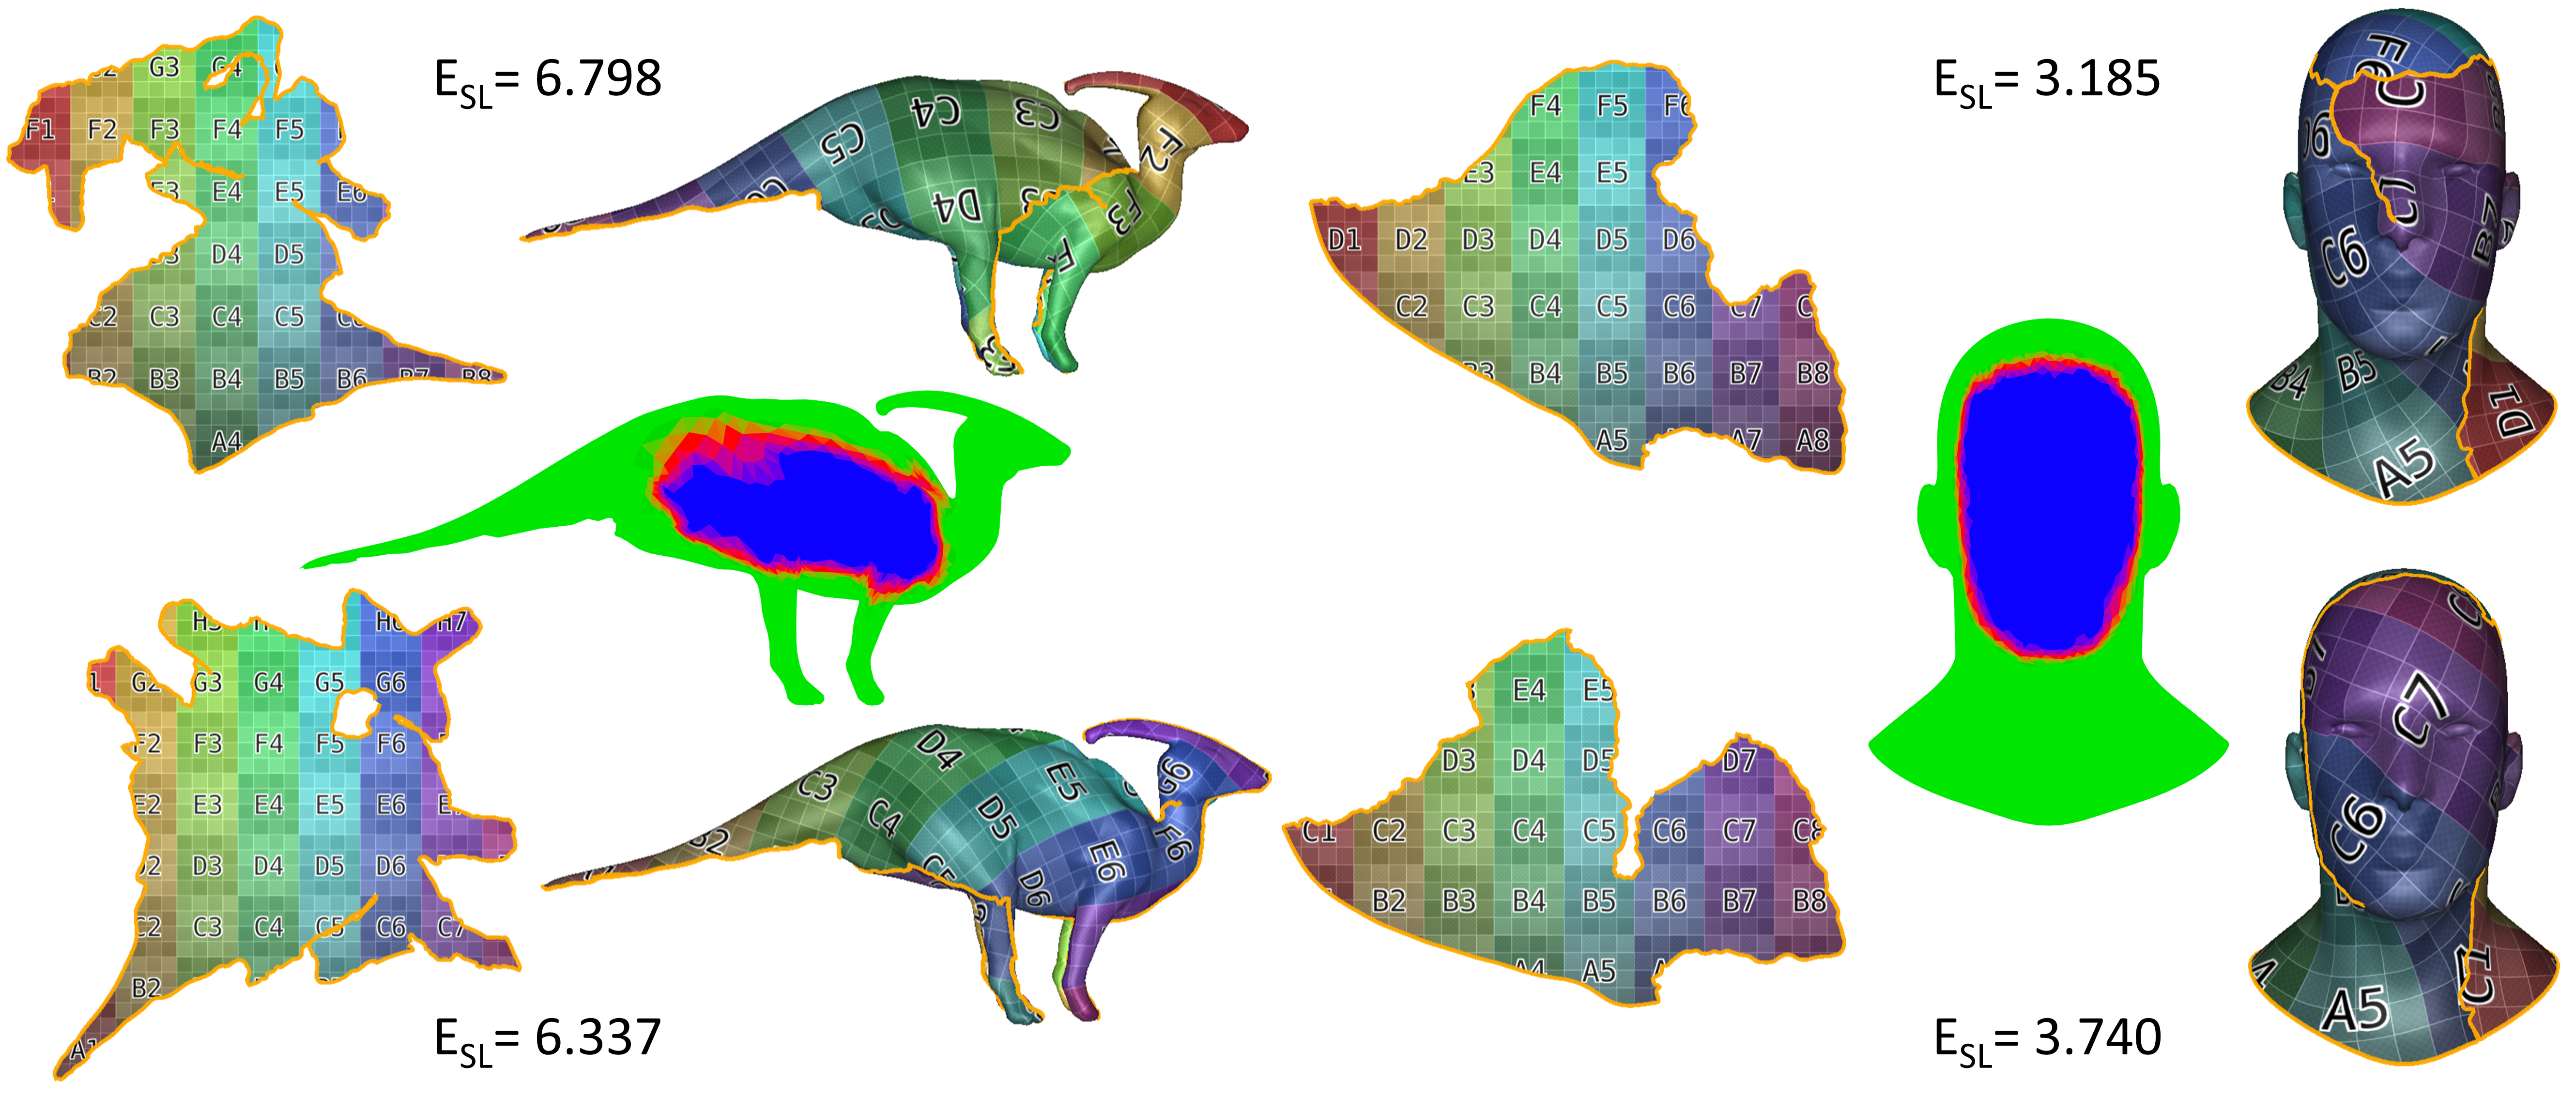
\includegraphics[width=\linewidth]{fig/regional_user.png}
\caption{Two examples with user-guided seam placement. The distortion bound is set to $b_d=4.1$ and we enforce bijectivity constraints in both cases. 
The fully automatic OptCut solution might place seams in salient regions (top), but the UV artist can paint ``do not cut here'' function (middle, blue), which will guide
the OptCut towards a better seam placement (bottom). Note that distortion and seam length is comparable in both cases. We happen to achieve shorter seams with additional user constraints for the dinosaur model since our method searches for a local optimum.}
\label{fig:regional_seam_placement}
\end{figure}

% \paragraph{Conformal Parameterization}
% Using a conformal energy~\cite{Hormann2000MIPS,Sheffer2005ABFPP} for $E_d$ will achieve joint seam placement and conformal parameterization. Figure~\ref{fig:conformal_vs_isometry} shows some results with $E_d = E_{ABForMIPS}$~\cite{} compared to results with $E_d = E_{d}$, where different seams are generated while our framework stays the same.

\paragraph{Alternative Cutting Strategy}
Our topology descent step leverages a small set of local topological operations to keep the framework simple and general. We also reduce the search complexity by filtering the candidates. Alternatively, one can use a richer set of more aggressive topological operations. For example, Geometry Images~\cite{Gu2002Geometry} leverage extrema-to-boundary cuts that connect the current boundary to the most distorted point (under current parameterization) using the shortest geodesic path. The advantage of this strategy is that it introduces more drastic topological updates at each iteration, potentially saving computational effort. We replace our topological search with this strategy (still terminating once $b_d$ is reached) and refer to the resulting variant of our method as EBCuts. As expected we found that the resulting approach is faster, but we found that it yields longer seams especially with tighter distortion bounds (Table~\ref{tb:comp_GI}) and for nearly-isometric UV maps where extremities are less prominent (Figure~\ref{fig:comp_GI}).
%\vova{We used notation $\mathcal{G}_T$ here, I don't think it appeared anywhere in the paper, so I removed it... we can define it earlier and bring it back if necessary...}

%The cutting strategy in the topology descent steps essentially build up the structure of the UV topology graph $\mathcal{G}_T$. By considering local topological operations, we built a dense graph connecting almost all the possible UV topologies and then reduce the search complexity by filtering. Alternatively, one can consider building $\mathcal{G}_T$ using only a sparse set of UV topologies and more aggressive topological operations, like the extremity-boundary (EBCuts) cut applied in Geometry Images~\cite{Gu2002Geometry}.


%We could alternatively apply EBCuts strategy in our framework without bijectivity constraints by simply alternating the cut with distortion minimization processes, and stop right after $b_d$ is reached. This variation of our method reaches identical distortion bounds with very similar seam length compared to our standard method, but is much faster since the EBCuts cut can be decided nearly instantly (Table~\ref{tb:comp_GI}). However, when we set smaller distortion bounds, the quality of the seams by EBCuts cut drops since extremities are not that obvious on a nearly isometric UV map (Figure~\ref{fig:comp_GI}).

\begin{table}[t]
\centering
\caption{Comparison between the standard OptCuts and using EBCuts cutting strategy in our framework, both without bijectivity constraints. We run the two methods on our benchmark and report statistics. EBCuts variant of our method is faster, but tends to produce longer seams.} 
\label{tb:comp_GI}
\begin{tabular}{|c|c|ccc|ccc|}
\hline
\multirow{2}{*}{$b_d$} & \multirow{2}{*}{strategy} & \multicolumn{3}{c|}{$E_{s}$} & \multicolumn{3}{c|}{time (s)} \\ \cline{3-8} 
                       &                         & avg      & min     & max      & avg       & min    & max      \\ \hline
\multirow{2}{*}{4.2}   & OptCuts                    & 3.819   & 0.080  & 14.545  & 87.0   & 0.3 & 417.8 \\
                       & EBCuts                & 3.868   & 0.159  & 14.929  & 13.0   & 0.1 & 72.1  \\ \hline
\multirow{2}{*}{4.1}   & OptCuts                    & 4.709   & 0.752  & 17.980  & 137.5  & 0.9 & 886.9 \\
                       & EBCuts                & 4.795   & 1.207  & 16.895  & 17.0   & 0.1 & 87.2  \\ \hline
\multirow{2}{*}{4.05}  & OptCuts                    & 6.142   & 0.277  & 21.566  & 213.2  & 3.9 & 1398.1   \\
                       & EBCuts                & 6.335   & 0.328  & 23.051  & 24.1   & 0.1 & 115.4 \\ \hline
\end{tabular}
\end{table}

\begin{figure}[t]
\centering
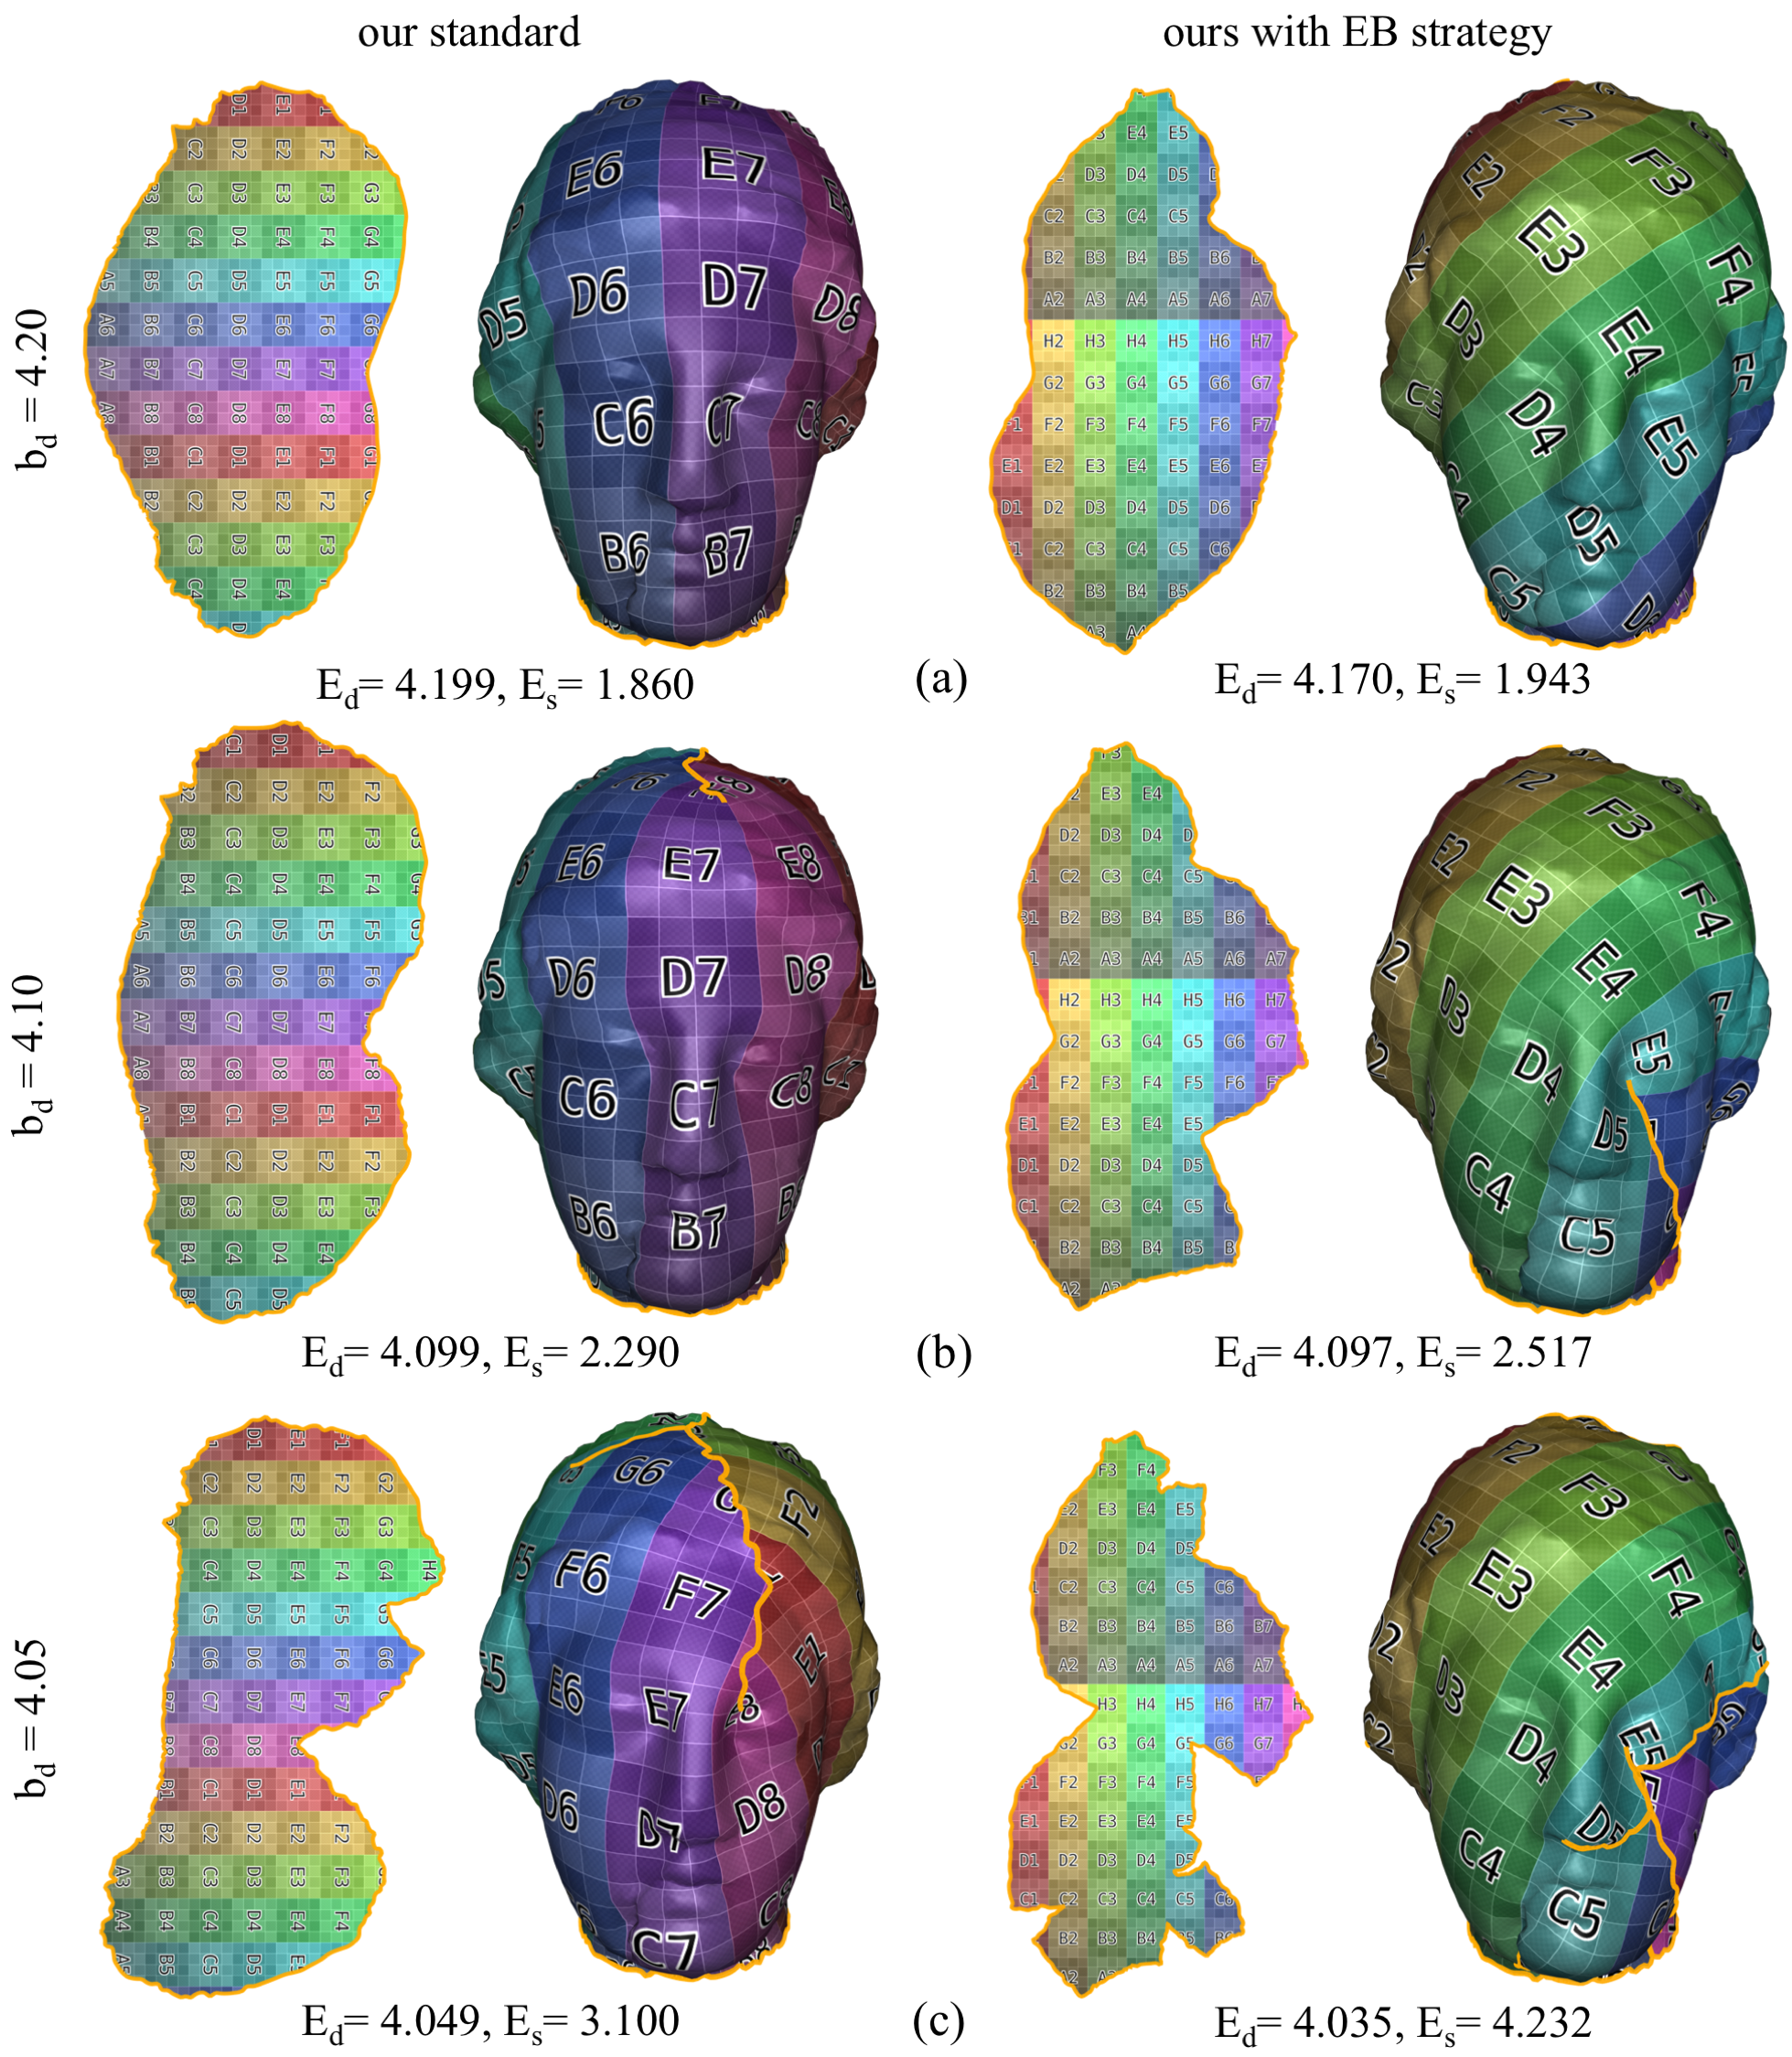
\includegraphics[width=0.8\linewidth]{fig/comp_GI.png}
\caption{Comparison between the standard OptCuts (left) and using EBCuts strategy in our framework (right), both without bijectivity constraints. EBCuts cutting strategy is very efficient in early stages (a, b), but it does not work well when the UV map gets closer to isometric where extremities are not very prominent (c).}
\label{fig:comp_GI}
\end{figure}
% also could be face_f10000, male_body_i_f10000, statue_4_i_f10000, statue_5_i_f10000, bimba_i_f10000

\paragraph{Warm Start}
Since our framework only provides local optima for a highly non-convex problem, initial conditions are relevant for the final result and computational cost. Several powerful topological heuristics have been used to provide a disk topology after cutting. %for the geometry optimization algorithm. 
We can consider any of these methods as a way to define an initialization for our approach. 

%Although we obtain high quality results given any initial embedding, the starting point does affect which local optimal point we will reach. Hence, it is meaningful to explore our method starting from initial seams with global observations. This will also benefit practical scenarios for improving preliminary UV maps while stay close to it.

As first example, we take the seams produced by our method with the EBCuts strategy and construct the initial embedding using our standard approach of Tutte's parameterization followed by distortion minimization. We can improve the seam quality while respecting the distortion bound by leveraging our local topological search which enables us to close unnecessary cuts by merging. Even with the bijectivity constraints, we still achieve shorter seam length (Figure~\ref{fig:comp_GI_outputAsInit}).

\begin{figure}[t]
\centering
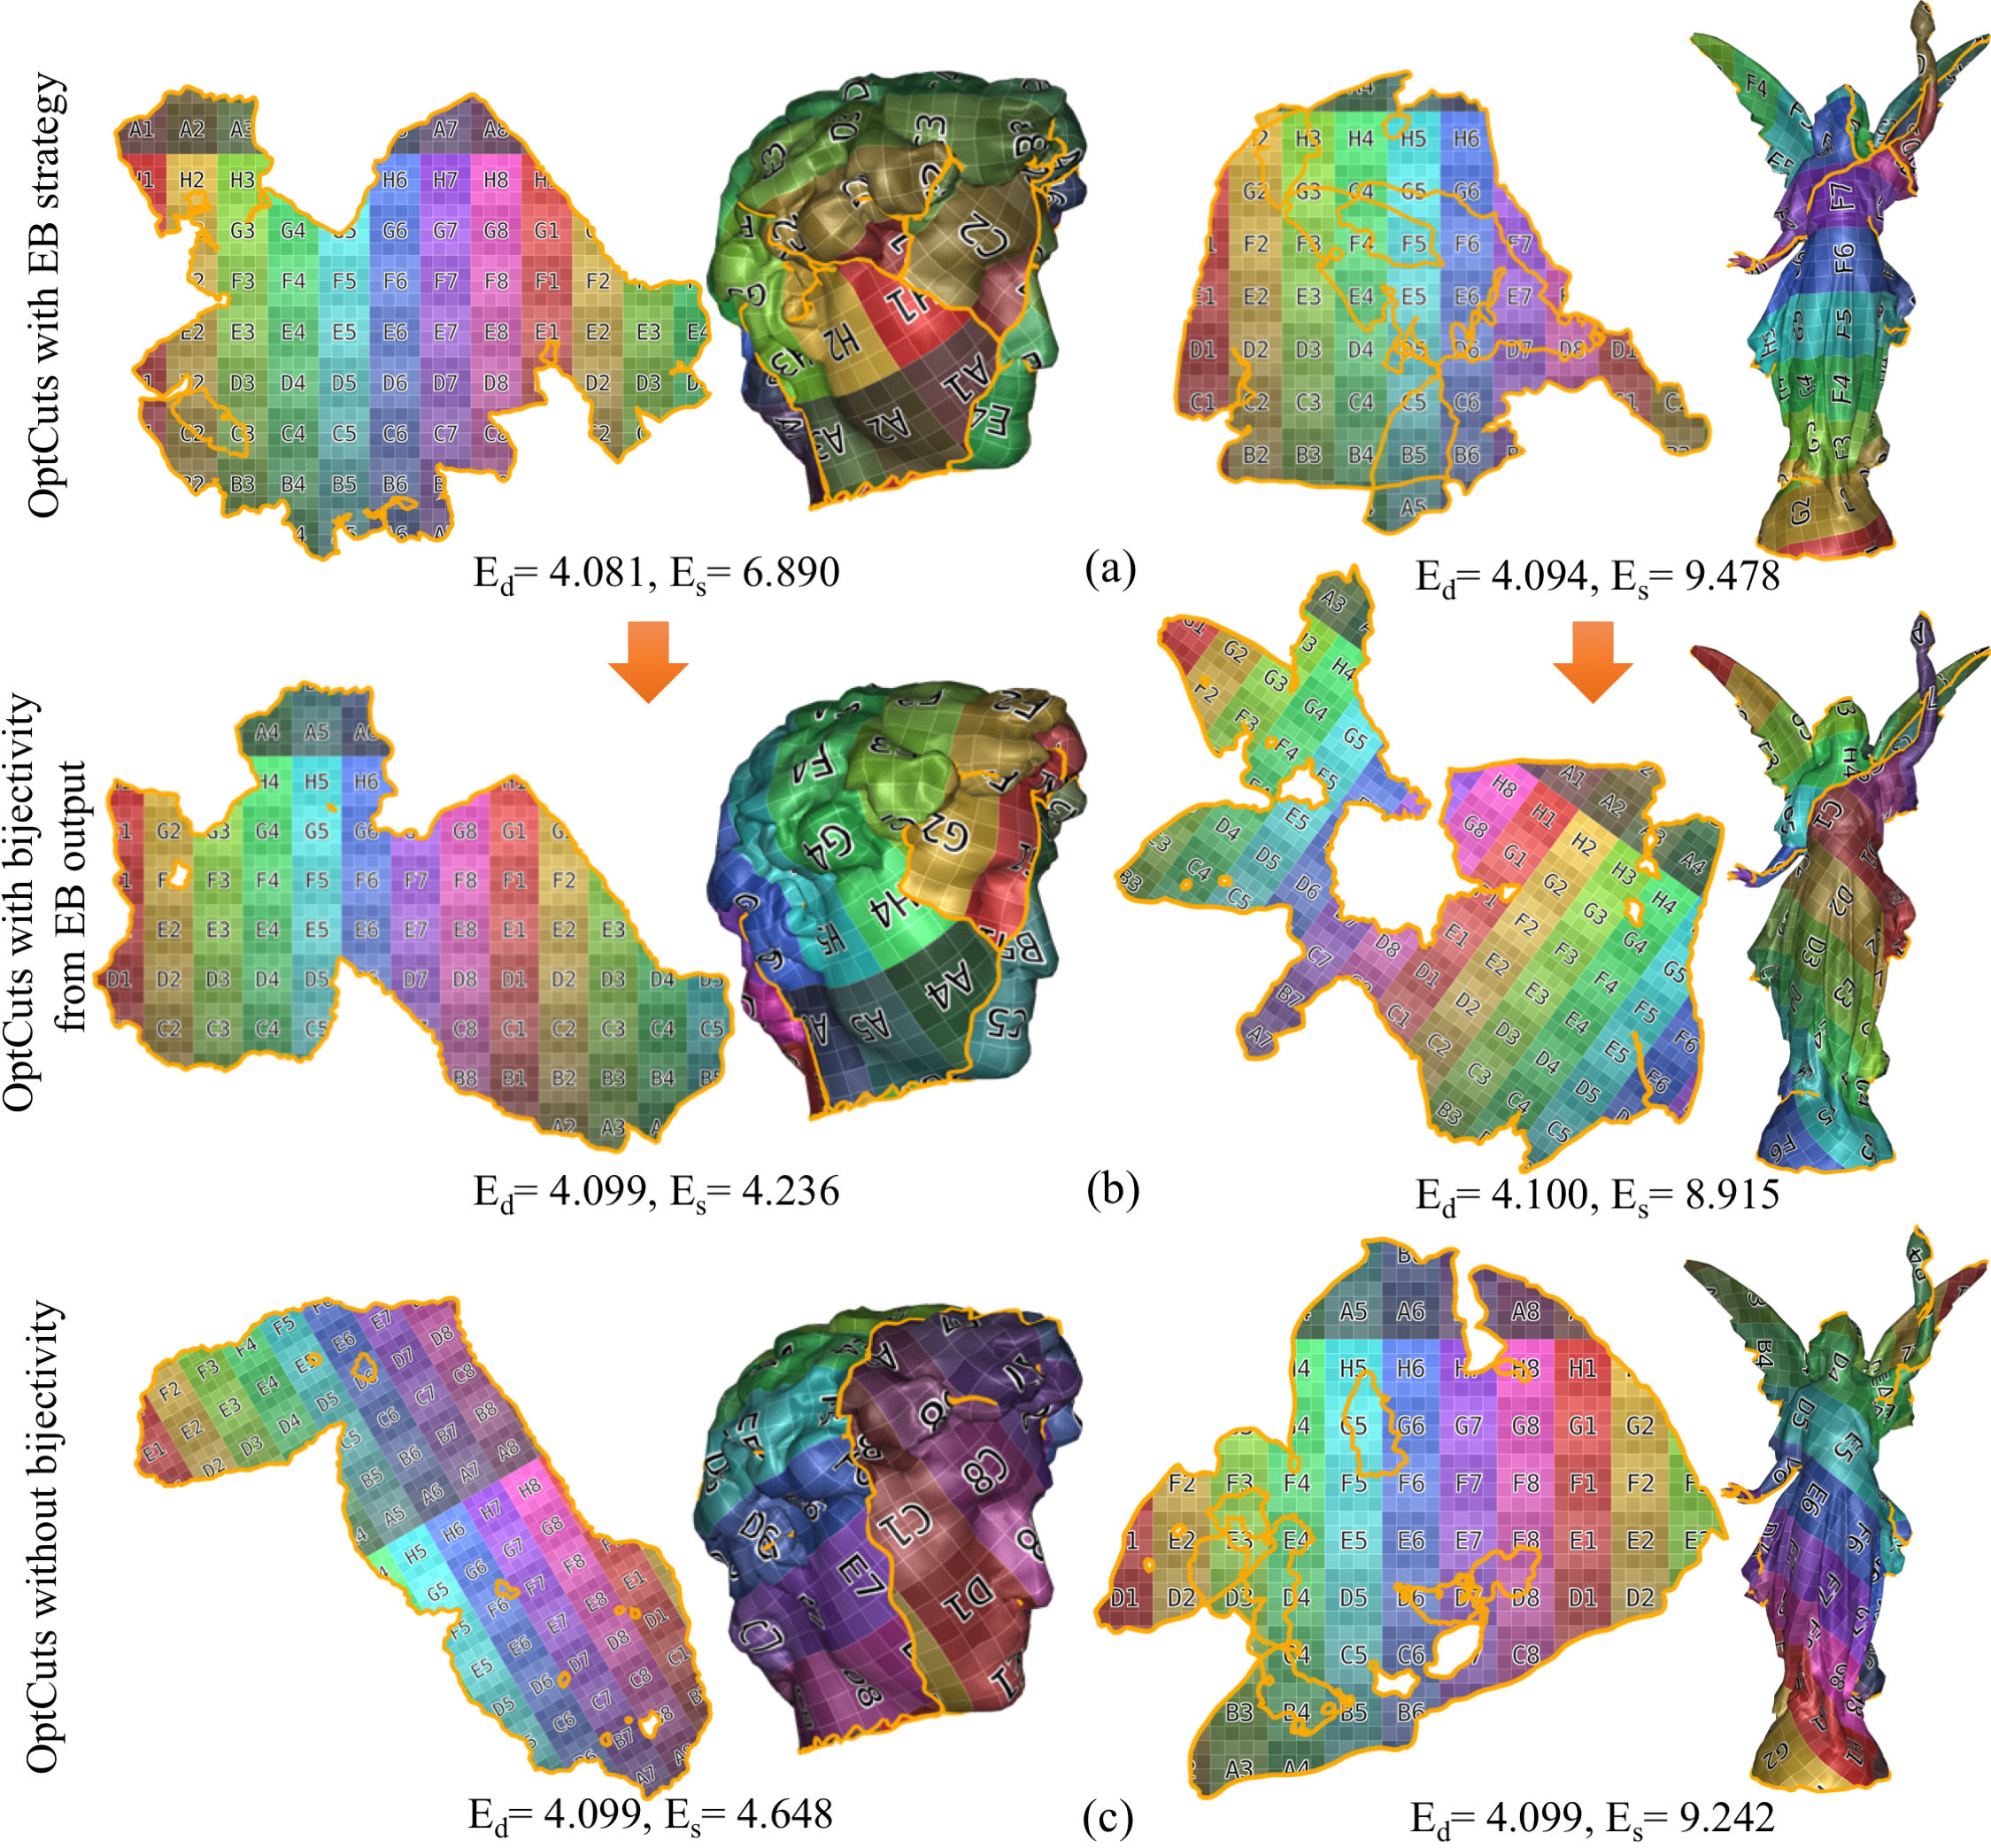
\includegraphics[width=\linewidth]{fig/comp_GI_outputAsInit.png}
\caption{We use the seams produced by our framework with EBCuts strategy at $b_d = 4.1$  initial UV map (a). We ran our OptCuts framework to improve the seam quality, reaching a locally optimal seam configuration under the given distortion bound even with bijectivity constraints (b). This seam length is also shorter than results obtained by standard OptCuts without bijectivity (c).}
\label{fig:comp_GI_outputAsInit}
\end{figure}
% also could be bimba, bunny

The second option we explore is Seamster~\cite{Sheffer2002Seamster}, a classic seam cutting strategy that detects local curvature extrema and connects them with a minimal spanning tree.  This approach can be sensitive to the user-set parameters such as size of surface regions for computing local extrema, which is a shape-dependent parameter that might require tuning. In this experiment, however, we pick two models that have been successfully cut with Seamster (a cow and a triceratops) and use our standard approach to produce the initial embedding, i.e., Tutte's embedding followed by minimizing $E_{d}$ with bijectvitiy constraints (Figure~\ref{fig:comp_Seamster}a). We use the resulting distortion as the upper bound and run the full OptCuts framework on the result. As demonstrated in Figure~\ref{fig:comp_Seamster}b, we achieve shorter seam length while maintaining the distortion bound and bijectivity. This seam length is also shorter than running our standard method without bijectivity from standard initialization (Figure~\ref{fig:comp_Seamster}c).

%With Seamster's best output seams on the cow and triceraptop model, we obtain UV maps by minimizing $E_{d}$ with bijectivity constraints (Figure~\ref{fig:comp_Seamster}a), and use them for warm start, setting their distortions as the upper bounds. As demonstrated in Figure~\ref{fig:comp_Seamster}b, we achieve shorter seam length while maintaining the distortion bound and bijectivity. This seam length is also shorter than running our standard method without bijectivity from standard initialization (Figure~\ref{fig:comp_Seamster}c).

\begin{figure}[t]
\centering
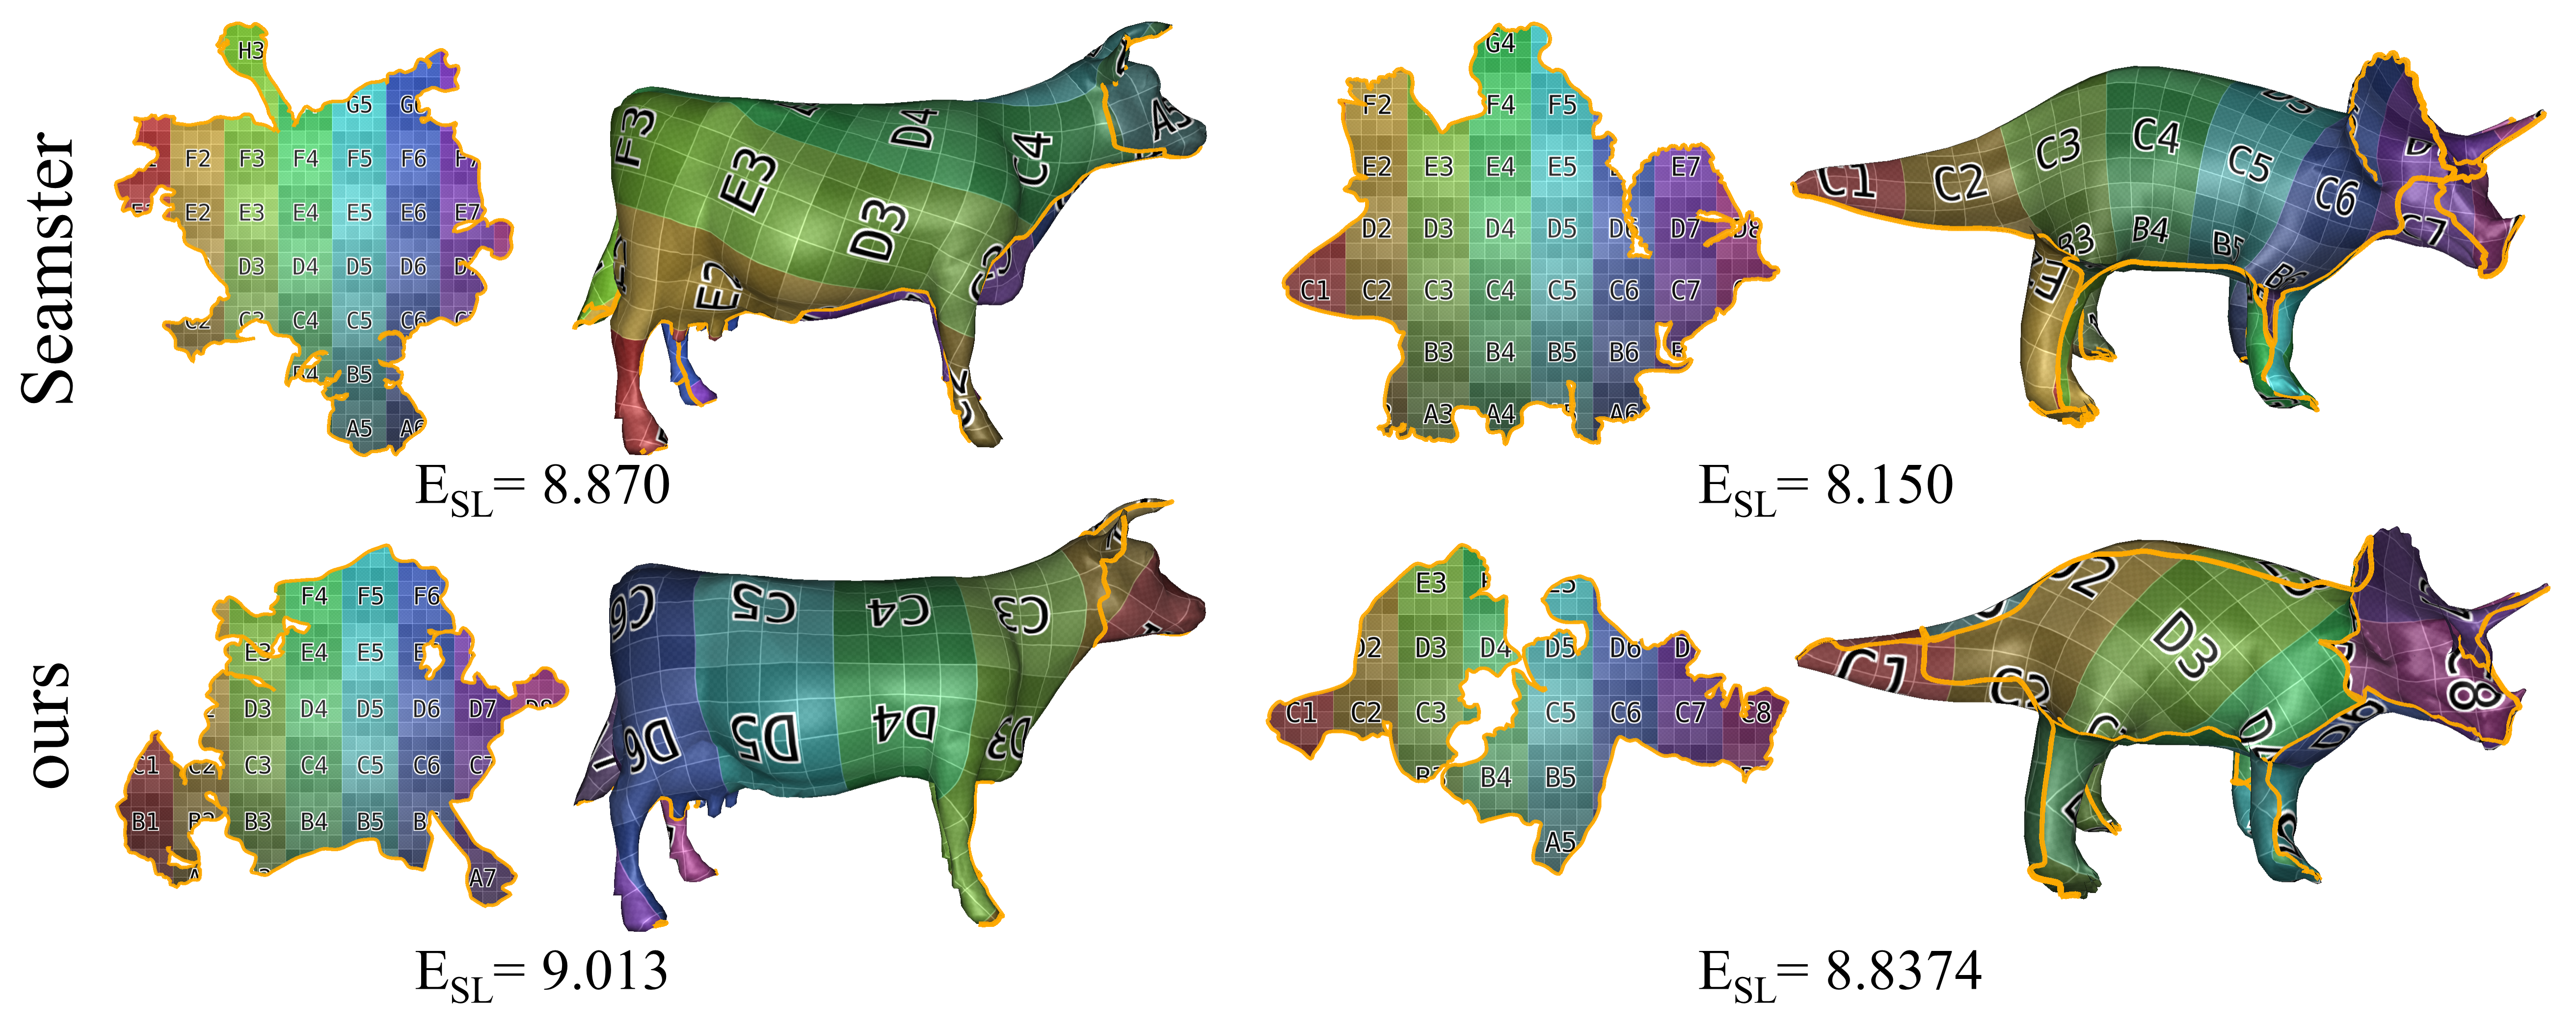
\includegraphics[width=\linewidth]{fig/comp_Seamster.png}
\caption{Starting from UV maps obtained by using Seamster's best output seams (a), we improve seam quality, reaching a locally optimal seam configuration while maintaining the distortion and bijectivity (b). This seam length is also shorter than running standard OptCuts without bijectivity from standard initialization (c).}
\label{fig:comp_Seamster}
\end{figure}

%For Seamster, user need to set the size of local regions for measuring extremity, which is a mesh and shape dependent parameter that requires fine tuning. Even OptCuts with standard initialization achieves similar seam length without any user assistance.



\section{Conclusions and Future Works}

take advantage of basic SIMD type of parallelism for accelerating query and improving results' quality by directly evaluating $f_v$ for neighbors and track multiple branches, very useful for practical implementations

if the user won't mind getting a slightly different triangulation, we could also create fractures in the interior of an element and locally remesh the stencil

start and solve in 3D by reducing curvature so that the need for locally injective initial embedding in parameterization problems could be eliminated, and the result is only "biased" by it's 3D shape, which is the most reasonable bias

try conformal energy like MIPS

bijectivity, seamless, and other augmentation of continuous energy?

handle user preferences on seam placement

seam smoothness, patch related discrete energy augmentation?

\section{Acknowledgements}

\bibliographystyle{ACM-Reference-Format}
\bibliography{OptCuts} 

\end{document}
